\documentclass[121pt, aspectratio=169, t]{beamer}
\usepackage[utf8]{inputenc}
\usepackage[brazil]{babel}
\usepackage{beamerthemesplit}

%-------------------------------------------------------------------------------
% --- Slide Justificado --------------------------------------------------------
\usepackage{ragged2e}
\usepackage{etoolbox}
\usepackage{soul}
\usepackage[normalem]{ulem}
\usepackage{cancel}
\usepackage{bm}
\usepackage{array}
\usepackage{wrapfig}
\apptocmd{\frame}{}{\justifying}{} % Allow optional arguments after frame.
\usepackage{amsmath,mathtools}
\usepackage{scrextend} % ajustar texto para direita

%\usepackage{enumitem}
%\usepackage{showframe}
% =============================================================================
% Pacotes para simbolos IPA
% =============================================================================
\usepackage{tipa}		% Simbolos do IPA
\usepackage{tipx}
%-------------------------------------------------------------------------------
% separação entre colunas e linhas de tabelas
\setlength{\tabcolsep}{2pt}
\renewcommand{\arraystretch}{1}
%-------------------------------------------------------------------------------
% Define a centralização de coluna com largura {|C{1 cm}|}
\newcolumntype{C}[1]{>{\centering\let\newline\\\arraybackslash\hspace{0pt}}m{#1}}
\newcolumntype{L}[1]{>{\raggedright\let\newline\\\arraybackslash\hspace{0pt}}m{#1}}
%-------------------------------------------------------------------------------
\newcommand\litem[1]{\item{\bfseries #1 }}
% --- Configuracoes de Tema e cores --------------------------------------------
\usetheme{CambridgeUS}

\definecolor{darkblue}{rgb}{0.07058,0.06470,0.01176}  % Preto 		RGB 21,20,16
\definecolor{yellow}{rgb}{0.57058,0.66470,0.71176}
\definecolor{myred}{rgb}{0.808,0.086,0.133}   % 0.98823,0.00000,0.00784
% amarelo	RGB (1,1,0.588224) 255,255,150 PAULA 4
\definecolor{myblue}{rgb}{0.57058,0.66470,0.71176} % azul 	RGB 13,29,174

\setbeamercolor{item}{fg=myblue}

\setbeamercolor{alerted text}{fg=yellow}
\setbeamercolor*{palette primary}{fg=darkblue,bg=yellow}
\setbeamercolor*{palette secondary}{fg=darkblue,bg=myred}
\setbeamercolor*{palette tertiary}{bg=darkblue,fg=yellow}
\setbeamercolor*{palette quaternary}{fg=darkblue,bg=yellow}

\setbeamercolor*{sidebar}{fg=darkblue,bg=orange!75!white}

\setbeamercolor*{palette sidebar primary}{fg=darkblue}
\setbeamercolor*{palette sidebar secondary}{fg=white}
\setbeamercolor*{palette sidebar tertiary}{fg=white} % darkblue!50!black
\setbeamercolor*{palette sidebar quaternary}{fg=white} % yellow!10!orange

\setbeamercolor*{titlelike}{parent=palette primary}
\setbeamercolor{frametitle}{bg=yellow}
\setbeamercolor{frametitle right}{bg=yellow}

\setbeamercolor*{separation line}{bg=myblue}
\setbeamercolor*{fine separation line}{bg=myblue}

\setbeamerfont*{frametitle}{size=\Large,
	series=\bfseries,
	parent=structure}

% --- Letras e simbolos matemáticos --------------------------------------------
% ------------------------------------------------------------------------------
\usepackage[bbgreekl]{mathbbol}  % Pacote para repreentação de conjuntos com \mathbb{R} com letras gregas
\usepackage{amsfonts}	% Pacote para repreentação de conjuntos com \mathbb{R}
\usepackage{mathrsfs}	% Pacote para letras matemáticas

\usepackage{amssymb} 	% diversos simbolos matematicos adicionais. Carrega automático com amsfonts
% ------------------------------------------------------------------------------
\usepackage{multicol}

\usepackage{multimedia}
\usepackage[]{graphicx}
\usepackage[]{color}

\usepackage{media9}

\usepackage{tabularx}
\usepackage{amsmath, amsthm, amssymb}
\usepackage{gensymb}
% --- Esta definicao deve vir antes --------------------------------------------
\usepackage{graphicx}			% Inclusão de gráficos
\usepackage{float}
% ------------------------------------------------------------------------------
\usefonttheme[onlymath]{serif}
\usepackage{hyperref}
\usepackage{multirow}
%\usepackage{subfig}
\usepackage{subcaption}
\usepackage{ragged2e}
%\captionsetup[subfigure]{labelformat=empty}
\usepackage{color}
\usepackage{colortbl}
\usepackage{textpos}


%---------------
\usepackage{tabularx}
\usepackage{booktabs}
\usepackage{multimedia}
\usepackage{tikz}
\usetikzlibrary{calc}
\usepackage{geometry}
\tikzset{
	invisible/.style={opacity=0},
	visible on/.style={alt={#1{}{invisible}}},
	alt/.code args={<#1>#2#3}{%
		\alt<#1>{\pgfkeysalso{#2}}{\pgfkeysalso{#3}} % \pgfkeysalso doesn't change the path
	},
}

\newenvironment{caixadireita}[2][.5\linewidth]
{\par\hfill\tabular{@{}p{#1}@{}}
	\multicolumn{1}{@{}c@{}}{#2} \\ }
{\endtabular\par}

% --- Desativando os botoes de navegacao ---------------------------------------
\setbeamertemplate{navigation symbols}{}
% --- Tela cheia ---------------------------------------------------------------
\hypersetup{pdfpagemode=FullScreen}
% --- Layout da pagina ---------------------------------------------------------
\hypersetup{pdfpagelayout=SinglePage}
% --- Relaxed footnotes --------------------------------------------------------
\newcommand{\lfr}[1]{\let\thefootnote\relax\footnote{\tiny #1}}
% --- Pasta com as imagens -----------------------------------------------------
\graphicspath{{Imagens/}}
% ------------------------------------------------------------------------------
% ==============================================================================
\title[SILF]{Modelagem estatística da variabilidade de inter e intrafalantes em fala contínua}
\author[Cantoni, M. M. \& Silva, A. P.]{Maria Mandes Cantoni\vspace{0cm} \& Adelino Pinheiro Silva\vspace{0cm}}
\institute[ADA]{\footnotesize{Núcleo de Linguística Computacional (ADA) / FALE/  UFMG} \\
	\footnotesize{Ciência e Inteligência de Dados para Gestão e Segurança Pública (CIDaGESP) / ACADEPOL/ PCMG} \vspace{0cm}}
\date{\today}
% ==============================================================================
\begin{document}
% ==============================================================================
\begin{frame}
	\begin{tikzpicture}[remember picture,overlay]
		\node[xshift=0cm,yshift=-1.25cm,opacity=1.0] at (current page.north) {
\includegraphics[height=1.5cm]{Headder_SILF.jpg}};
	\end{tikzpicture}
	\vspace{0.25cm}
	\titlepage
	\vspace{-0.5cm}
	\begin{tikzpicture}[remember picture,overlay]
		\node[xshift=3.34cm,yshift=-3.25cm,opacity=1.0] at (current page.west) {
\includegraphics[height=1.25cm]{ADA_logo-borda.png}};
		\node[xshift=-1.125cm,yshift=-3.25cm,opacity=1.0] at (current page.east) {
\includegraphics[height=1.25cm]{logo_Acadepol_02.png}};
	\end{tikzpicture}
\end{frame}
% ==== Sumário =================================================================
\section{Sumário}
\begin{frame}
	\frametitle{Sumário}
	\tableofcontents
\end{frame}
% ==============================================================================
\AtBeginSection[]
{
	\begin{frame}
		\frametitle{Assuntos}
		\tableofcontents[currentsection]
	\end{frame}
}
% ==== Introdução ==============================================================
\section{Introdução}
% ------------------------------------------------------------------------------
\begin{frame}[fragile=singleslide]
	\frametitle{Informação no sinal de fala}
	\begin{itemize}[]
		\item Codificação;
		\item identidade de grupo \cite{Labov1973};
		\item identidade do falante \cite{Doddington2001, Ishihara2021}
		\item condições do falante;
		\item contexto fonológico...
	\end{itemize}
	\vspace{0.75cm}
	\begin{itemize}[]
		\item Fonatórios (pregas vocais); e
		\item Articulatórios (trato vocal). \cite{Fant1971,Flanagan2013}.
	\end{itemize}

	\begin{tikzpicture}[remember picture,overlay]
		\node[xshift=-4.0cm,yshift=0.75cm,opacity=1.0] at (current page.east) {
\includegraphics[width=7.5cm]{3381-scaled-e1707509515966.jpg}};
	\end{tikzpicture}
	\vfill
	\lfr{Imagem: \url{https://www.umsabadoqualquer.com/quem-realmente-deveria-estar-morto/}}
\end{frame}
% ------------------------------------------------------------------------------
\begin{frame}[fragile=singleslide]
	\frametitle{Variabilidade intra e extrafalante} 
	\vspace{0.25cm}
	\textbf{Intrafalante} presente na fala de um mesmo locutor, devido as diferenças de como os movimentos da fala são articulados por ele;
	\vspace{0.75cm}
	
	\textbf{Extrafalante}: observada entre falantes distintos devido a diferentes tratos vocais e habilidades motoras \cite{Kilbourn-Ceron2021}.
	\begin{tikzpicture}[remember picture,overlay]
		\node[xshift= 4.0cm,yshift=-2.5cm,opacity=1.0] at (current page.west) {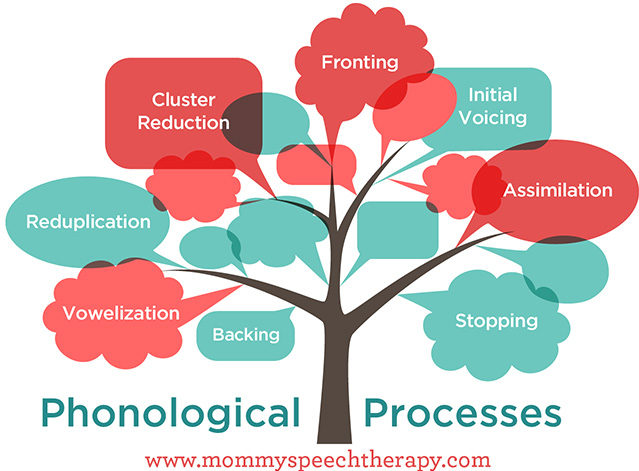
\includegraphics[height=2cm]{PhP.png}};
		\node[xshift=-4.0cm,yshift=-2.5cm,opacity=1.0] at (current page.east) {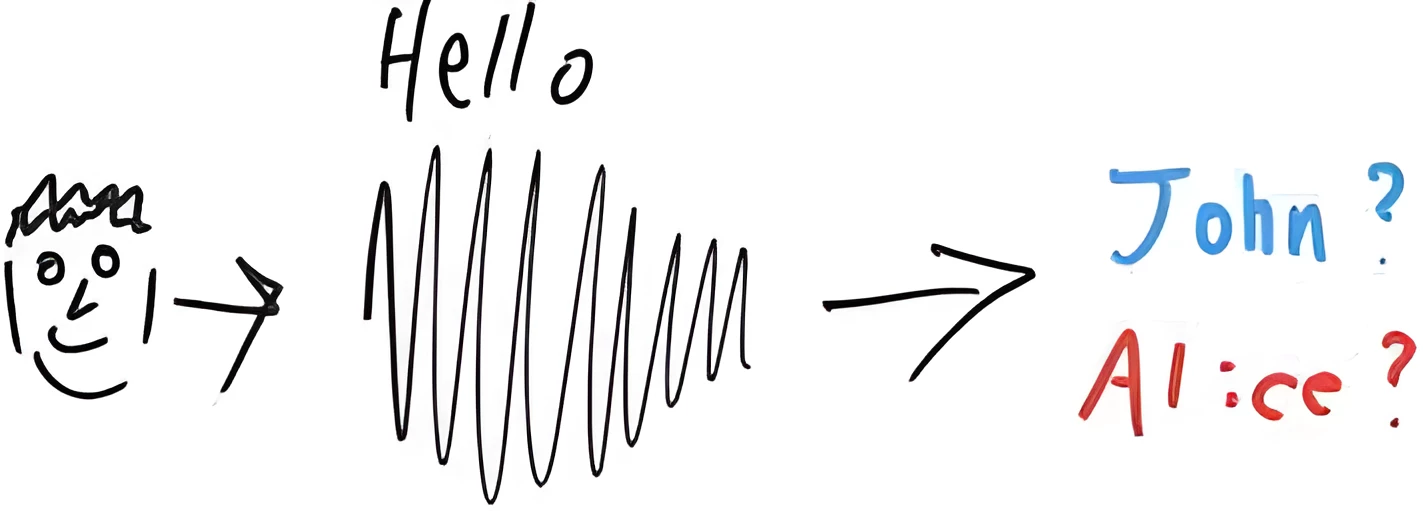
\includegraphics[height=2cm]{SR.png}};
	\end{tikzpicture}
	\vfill
	\lfr{Imagens: \url{https://mommyspeechtherapy.com/?p=2158} e \url{https://aruno14.medium.com/speaker-recognition-using-tensorflow-1f007c2a7702}}
\end{frame}
% ------------------------------------------------------------------------------
\begin{frame}[fragile=singleslide]
	\frametitle{Objetivo, perguntas e hipótese} 
	\textbf{Objetivo:} modelar a variabilidade relacionada ao falante, consideram-se os papéis das estruturas articulatórias e vocais a partir de fala contínua. \\
	\vspace{0.5cm}
	\textbf{Perguntas:}
	\begin{enumerate}
		\item Quanto a variação do falante se deve a diferenças articulatórias e quanto se deve a diferenças de voz? 
		\item Quais medidas acústicas são mais robustas para classificação de falantes em fala contínua? 
	\end{enumerate}
	\vspace{0.5cm}
	\textbf{Hipótese:} Um modelo linear generalizado pode remover informação do contexto fonológico e com isso acentuar a identidade do locutor. \\
	\vspace{0.5cm}
	\textbf{Restrição:} Modelagem estatística no espaço mensurável para ter mais controle e transparência em contraponto a RNA~\cite{McQuisten2009,Wuethrich2019}.
\end{frame}
% ==============================================================================
\section{Materiais e métodos}
\begin{frame}[fragile=singleslide]
	\frametitle{Base de dados e aplicações}
	\begin{itemize}[]
		\item 18 locutores (8 F e 10 M) do corpus CEFALA 1 \cite{Neto2019};
		\item 5615 unidades distribuídas em 64 categorias, sendo 12 vogais e 52 ditongos;
		\item entre 143 e 512 unidades por locutor;
		\item rotulagem manual em TextGrid no \textit{praat} com revisão;
		\item processamento em \textit{python 3.11} com pacotes \textit{scipy}, \textit{scikit-learn}, \textit{pandas} e \textit{matplotlib}.
	\end{itemize}

	\begin{tikzpicture}[remember picture,overlay]
		\node[xshift=0.0cm,yshift=-2.25cm,opacity=1.0] at (current page.center) {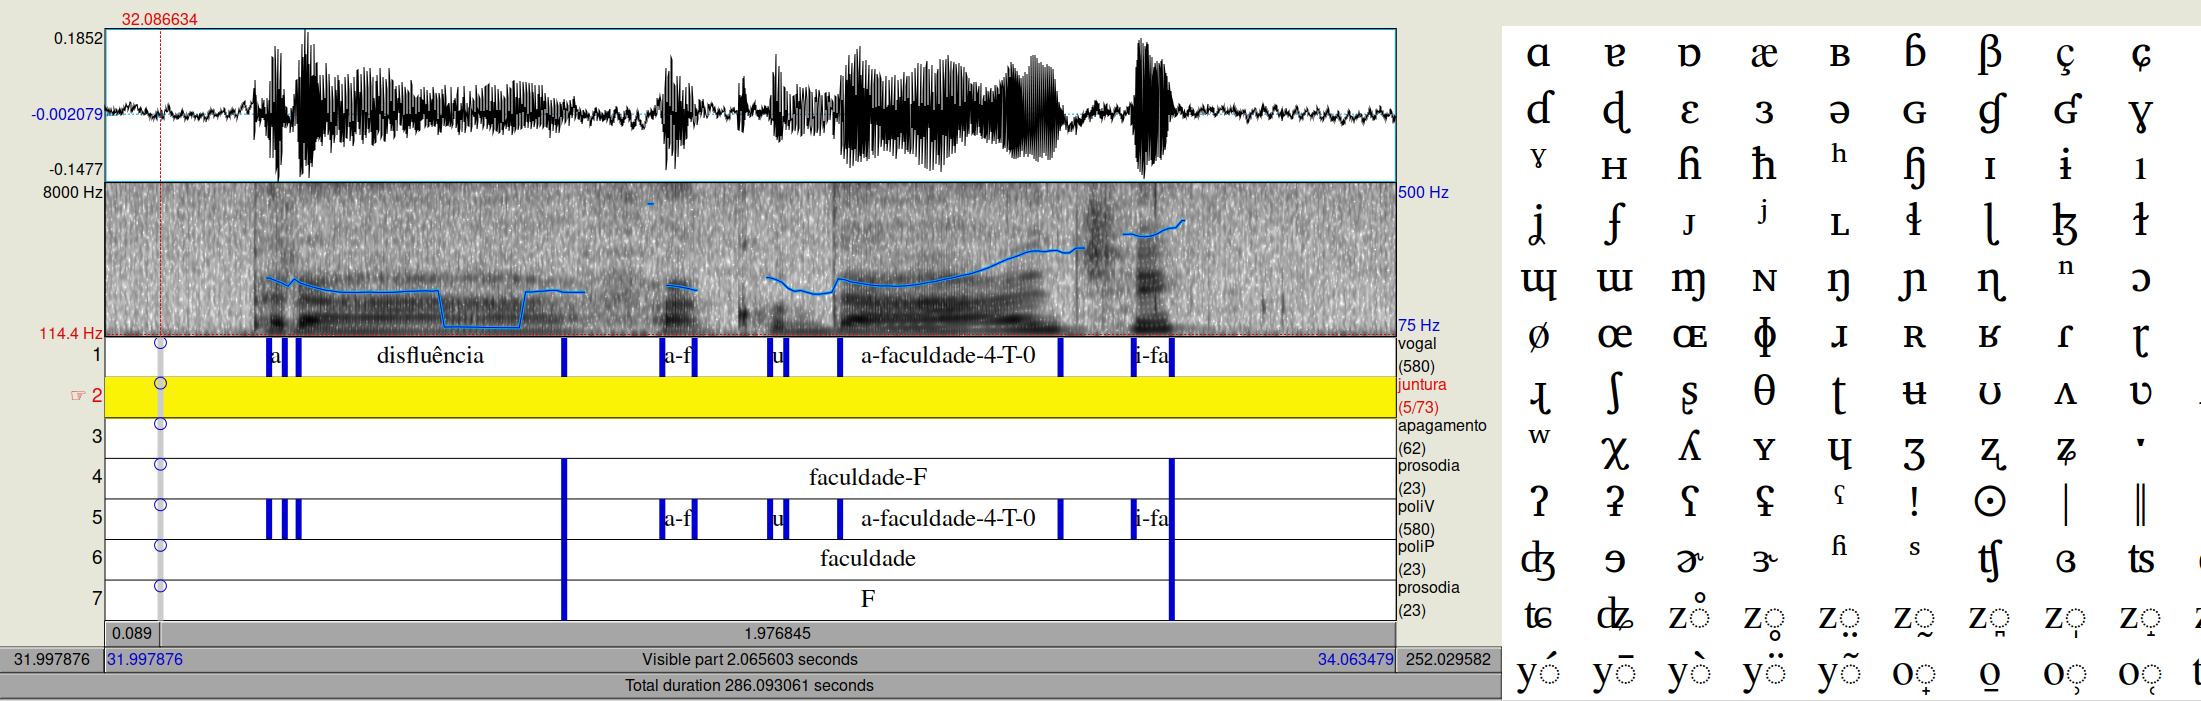
\includegraphics[height=3.5cm]{Praat-TextGrid.png}};
	\end{tikzpicture}
%	\vfill
%	\lfr{Imagem: \url{Praat-TextGrid.png}}
\end{frame}
% ------------------------------------------------------------------------------
\begin{frame}[fragile=singleslide]
	\frametitle{Distribuição das unidades amostrais}
	\begin{figure}
		\centering
%		\caption{}
		\begin{subfigure}[t]{8.5cm}
%			\centering
			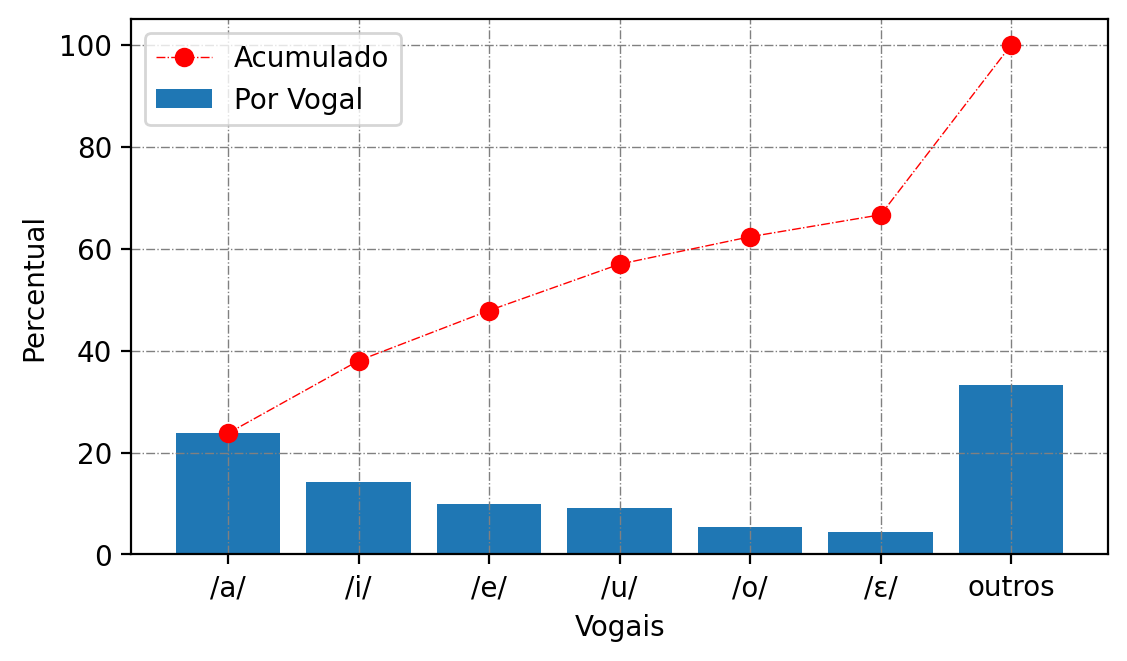
\includegraphics[height=5.9cm]{Vowels_Count.png}
			\caption{Percentual de ocorrência das unidades amostrais.}
%			\label{fig:Imagem_01}
		\end{subfigure}
		\hfill
		\begin{subfigure}[t]{4.75cm}
			\centering
			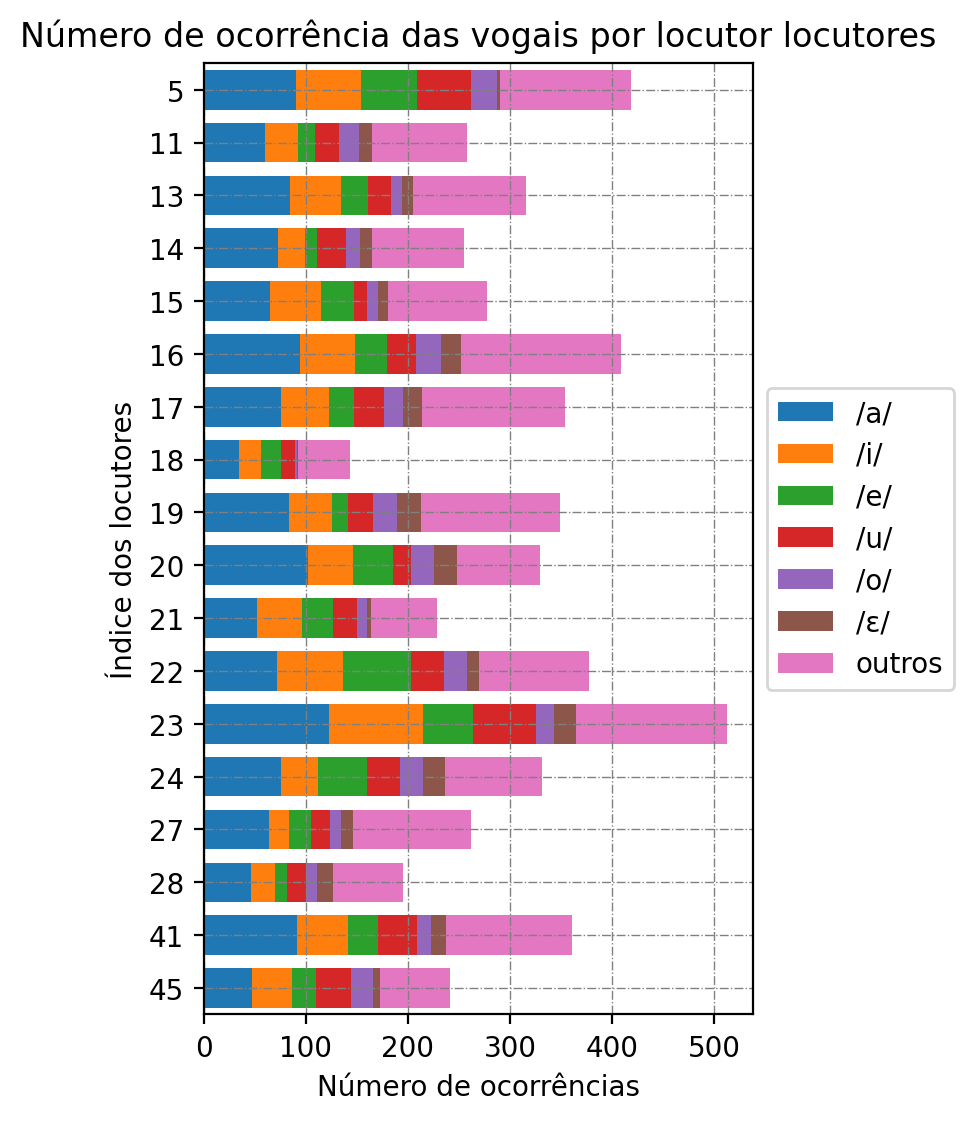
\includegraphics[height=5.9cm]{PLT_01_Sons_Contexto.png}
			\caption{Ocorrência das unidades amostrais por locutor.}
%			\label{fig:Imagem_02}
		\end{subfigure}
	\end{figure}

%	\begin{tikzpicture}[remember picture,overlay]
%		\node[xshift=-2.95cm,yshift=-1.0cm,opacity=1.0] at (current page.center) {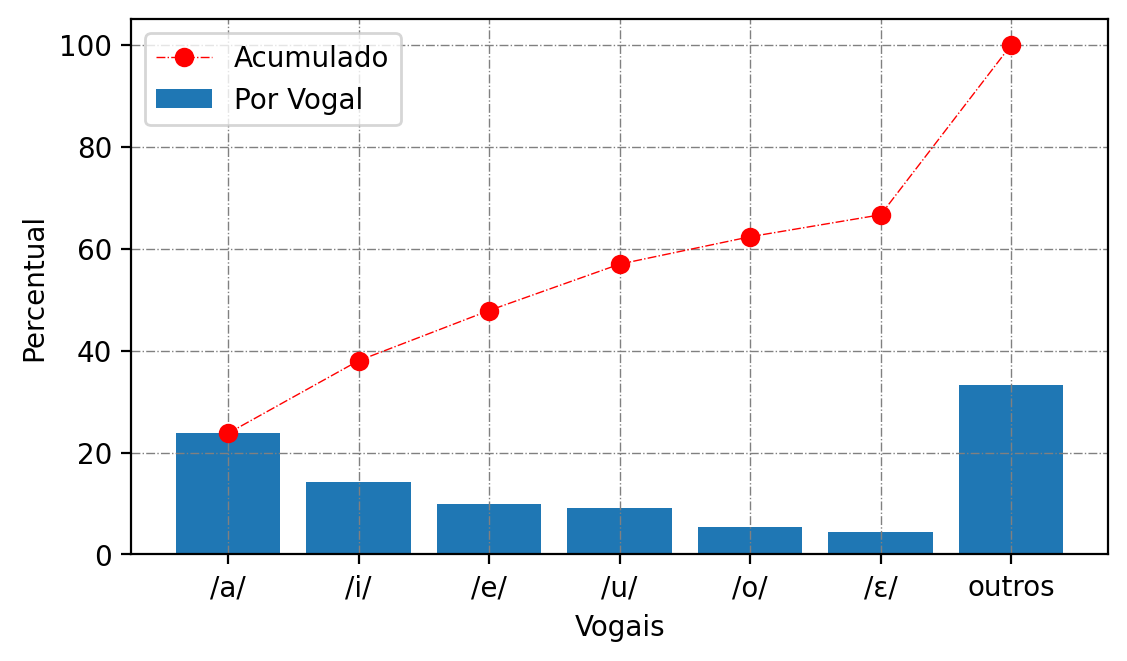
\includegraphics[height=6.0cm]{Vowels_Count.png}};
%		\node[xshift=5.05cm,yshift=-1.0cm,opacity=1.0] at (current page.center) {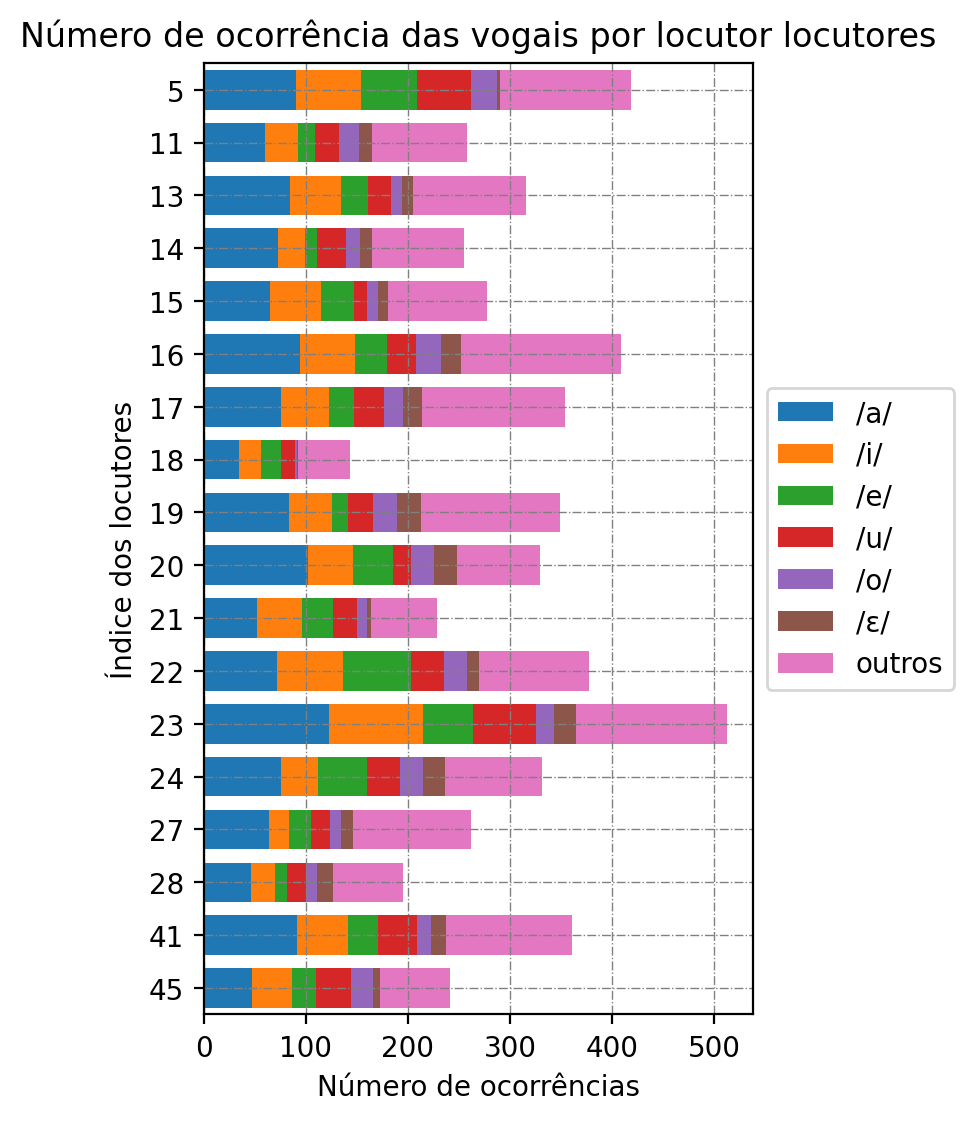
\includegraphics[height=6.0cm]{PLT_01_Sons_Contexto.png}};
%	\end{tikzpicture}
\end{frame}

% ------------------------------------------------------------------------------
\begin{frame}[fragile=singleslide]
	\frametitle{Variáveis de contexto}
	\begin{table}[]
		\small
		\begin{tabular}{L{3.5cm}|L{11cm}}
			\toprule
			Variável             & Descrição \\ \midrule
			Sexo do falante      & Feminino ou masculino.\\
			Tonicidade da sílaba & Posição relativa da sílaba em relação a tônica, os valores variam entre tônica, pré-tônica ou pós-tônica. \\
			Posição na palavra   & Sílaba da palavra, a partir do começo, a vogal se encontra. Os valores na amostra variam entre 0 e 6. \\
			Ditongação           & Indica se a unidade amostral é uma vogal com valor 0 ou ditongo com valor 1. \\
			Fechamento           & Sílaba onde se encontra a vogal (ou ditongo) é fechada por consoante.  \\
			Som anterior         & Som fonológico que ocorre antes da vogal, valor nulo (final de palavra), vogal (e.g., /a/, /\textepsilon /, /ĩ/, ...) ou consoante (e.g., /p/, /\textteshlig/, /n/, ...). \\
			Som posterior        & Som fonológico que ocorre depois da vogal, valor nulo (final de palavra), vogal (e.g., /a/, /\textepsilon /, /ĩ/, ...) ou consoante (e.g., /p/, /\textteshlig/, /n/, ...). \\ \bottomrule
		\end{tabular}
	\end{table}
\end{frame}
% ------------------------------------------------------------------------------
\begin{frame}[fragile=singleslide]
	\frametitle{Medidas acústicas}
	\begin{table}[]
		\caption{Lista de medidas conforme análise de \cite{Lee2019}.}
		\small
		\begin{tabular}{L{4cm}|L{4cm}|L{3.5cm}|L{3cm}}
			\toprule
			Tipo de medida acústica & Tendência central   & Variabilidade    & Categoria    \\ \midrule
			1 – Intensidade e duração     & Intensidade, Duração   & --   & Não classificada \\
			\begin{tabular}[c]{@{}l@{}}2 - Frequência dos\\ formantes\end{tabular} & \begin{tabular}[c]{@{}l@{}}média $F_1$, média $F_2$,\\ média $F_3$, média $F_4$ e\\ média $F_D$\end{tabular} & \begin{tabular}[c]{@{}l@{}}Cov $F_1$, Cov $F_2$,\\ Cov $F_3$, Cov $F_4$ e\\ Cov $F_D$\end{tabular} & Articulatória    \\
			3 - Frequência fundamental    & média $F_0$  & Cov  $F_0$   & Vocal  \\
			4 - Forma espectral da fonte harmônica   & média H1*–H2*, média H2*–H4*, média  H4*–H2kHz* e média H2kHz*–H5kHz  & Cov H1*–H2*, Cov H2*–H4*, Cov H4*–H2kHz* e Cov H2kHz*–H5kHz & Vocal  \\
			5 - Ruído espectral/fonte inarmônica & média CPP e média SHR  & Cov CPP e Cov SHR  & Vocal  \\ \bottomrule
		\end{tabular}
	\end{table}
\end{frame}
% ++++++++++++++++++++++++++++++++++++++++++++++++++++++++++++++++++++++++++++++
\subsection{Análise de componentes principais}
% ------------------------------------------------------------------------------
\begin{frame}[fragile=singleslide]
	\frametitle{Distribuição das componentes principais}
		\begin{figure}
		\centering
		%		\caption{}
		\begin{subfigure}[t]{8.2cm}
			%			\centering
			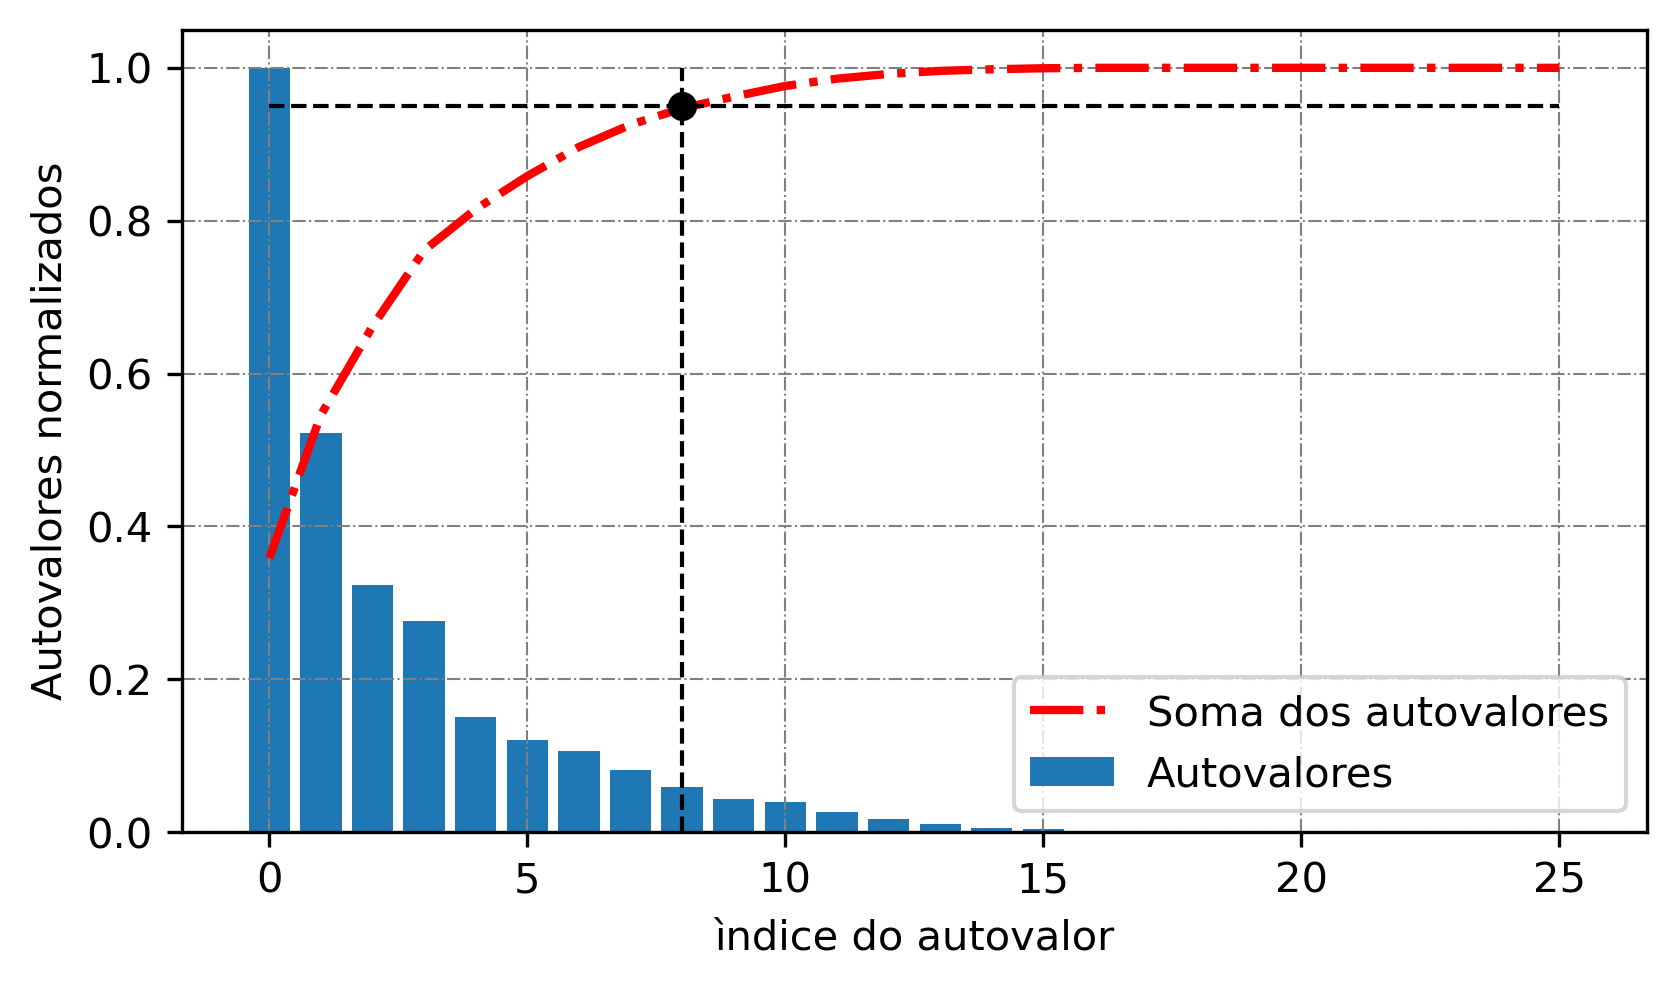
\includegraphics[height=5.2cm]{EiVals_features.png}
			\caption{Autovalores normalizados da matriz de correlação.}
			%			\label{fig:Imagem_01}
		\end{subfigure}
		\hfill
		\begin{subfigure}[t]{5.9cm}
			\centering
			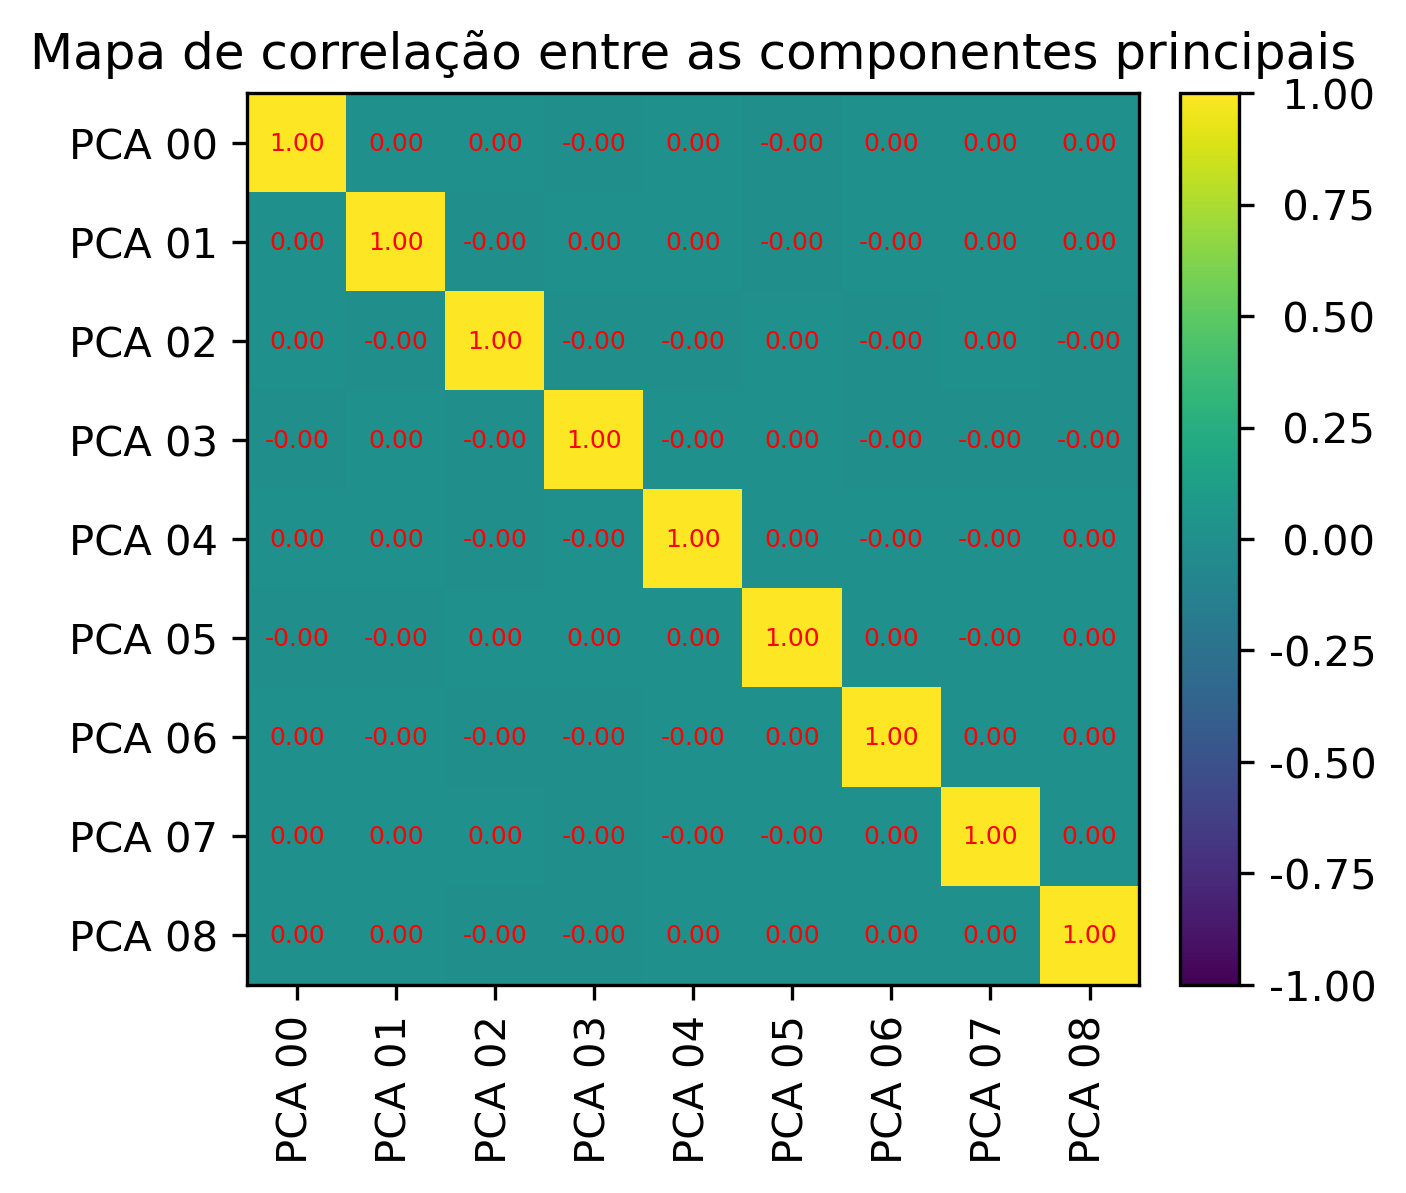
\includegraphics[height=5.2cm]{Correelacao_pca.png}
			\caption{Mapa de correlação entre as nove primeiras CP.}
			%			\label{fig:Imagem_02}
		\end{subfigure}
	\end{figure}
\end{frame}
% ------------------------------------------------------------------------------
\begin{frame}[fragile=singleslide]
	\frametitle{Correlação no espaço de componentes principais}
	\begin{figure}
		\centering
		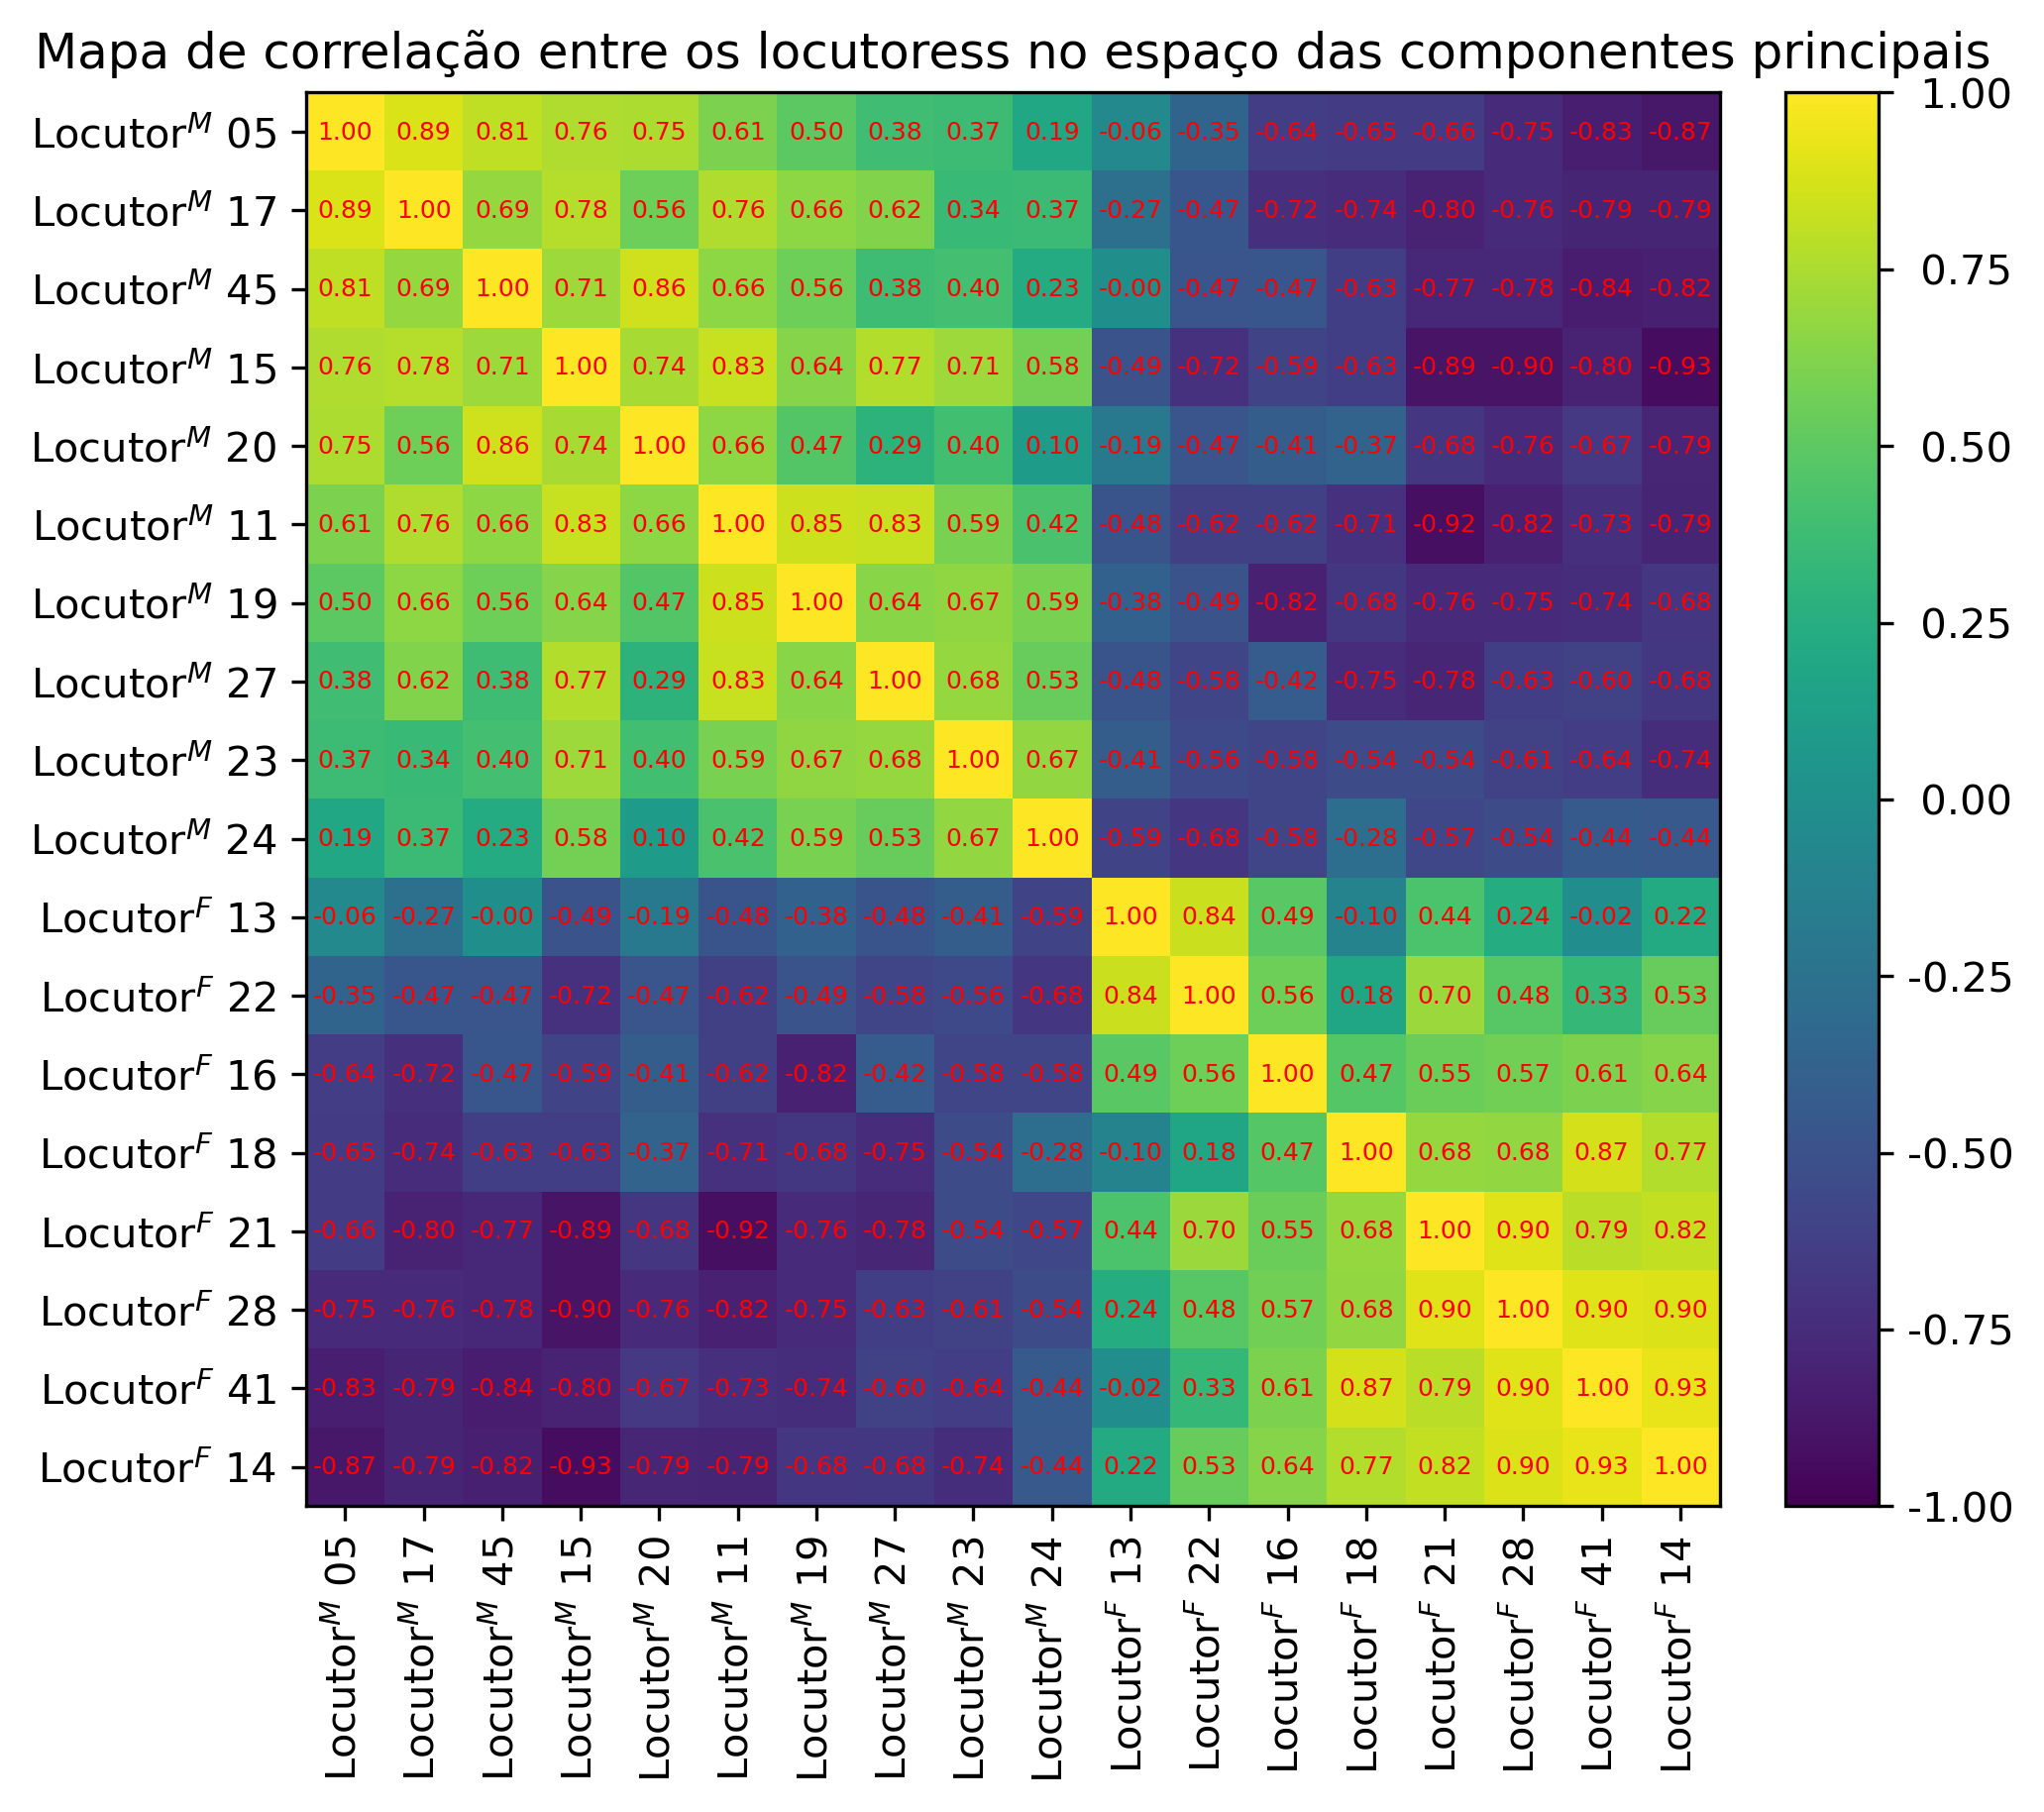
\includegraphics[height=7cm]{Correelacao_pca_loc.png}
		%		\caption{Autovalores normalizados da matriz de correlação.}
	\end{figure}
\end{frame}
% ==============================================================================
\section{Metodologia de modelagem e resultados}
\subsection{Descrição Procedimental}
\begin{frame}[fragile=singleslide]
	\frametitle{Equacionamento}
	\textbf{Modelos linear generalizado} (GLM - \textit{generalized linear model})
	
	\begin{equation}
		 Y_{n} \approx X_{C|n} + X_{L|n} + \epsilon_{n}
	\end{equation}

	\begin{equation}
		Y_{n} \approx X_{CM|n} + X_{CN|n} + X_{L|n} + \epsilon_{n} \approx X_{CM|n} + \epsilon_{L,CN|n}
	\end{equation}

	\begin{eqnarray}
		\bar{Y}_{n} &=& \beta_{0} +  \mathbf{B} \cdot \mathbf{X}_{CM|n} \nonumber \\
		Y_{n} &=& \mathcal{N} \left( \bar{Y}_{n} ,\epsilon_{L,CN|n} \right) 
	\end{eqnarray}

\end{frame}

\begin{frame}[fragile=singleslide]
	\frametitle{Criação de variáveis fictícias}
	Número de Categorias dos sons anteriores e posteriores\\
	
	Homogeneizar a ocorrência em todos os locutores\\
	
	\begin{enumerate}
		\item Obstrução: valor 1 para vogais e 0 para consoantes.
		\item Vozeamento: em todas vogais e nas consoantes vozeadas é 1 e 0 nos sons não
		vozeados.
		\item Abertura da boca: Valor 0 para as vogais altas e para as consoantes plosivas e 1 caso contrário.
		\item Posição dos articuladores: Apresenta valor 1 para as consoantes articuladas na posição frontal da boca (i.e., lábios, dentes ou alvéolo) e para as vogais frontais.
		\item Nasalidade: apresenta valor 1 para as vogais e consoantes nasais.
	\end{enumerate}
	Em caso de ausência de som anterior ou precedente todas as variáveis fictícias assumem valor igual a 0.
\end{frame}

\begin{frame}[fragile=singleslide]
	\frametitle{Ajuste do modelo}
	\begin{columns}
		\begin{column}{0.25\textwidth}
			Conjunto de treinamento (70\%) e de teste (30\%).\\
			\vspace{0.5cm}
			Homogenização de 20 vetores por locutor (14/6) por \textit{bootstrap}.
		\end{column}
		\begin{column}{0.75\textwidth}  %%<--- here	
				\vspace{-1.5cm}
				\begin{figure}
				\centering
				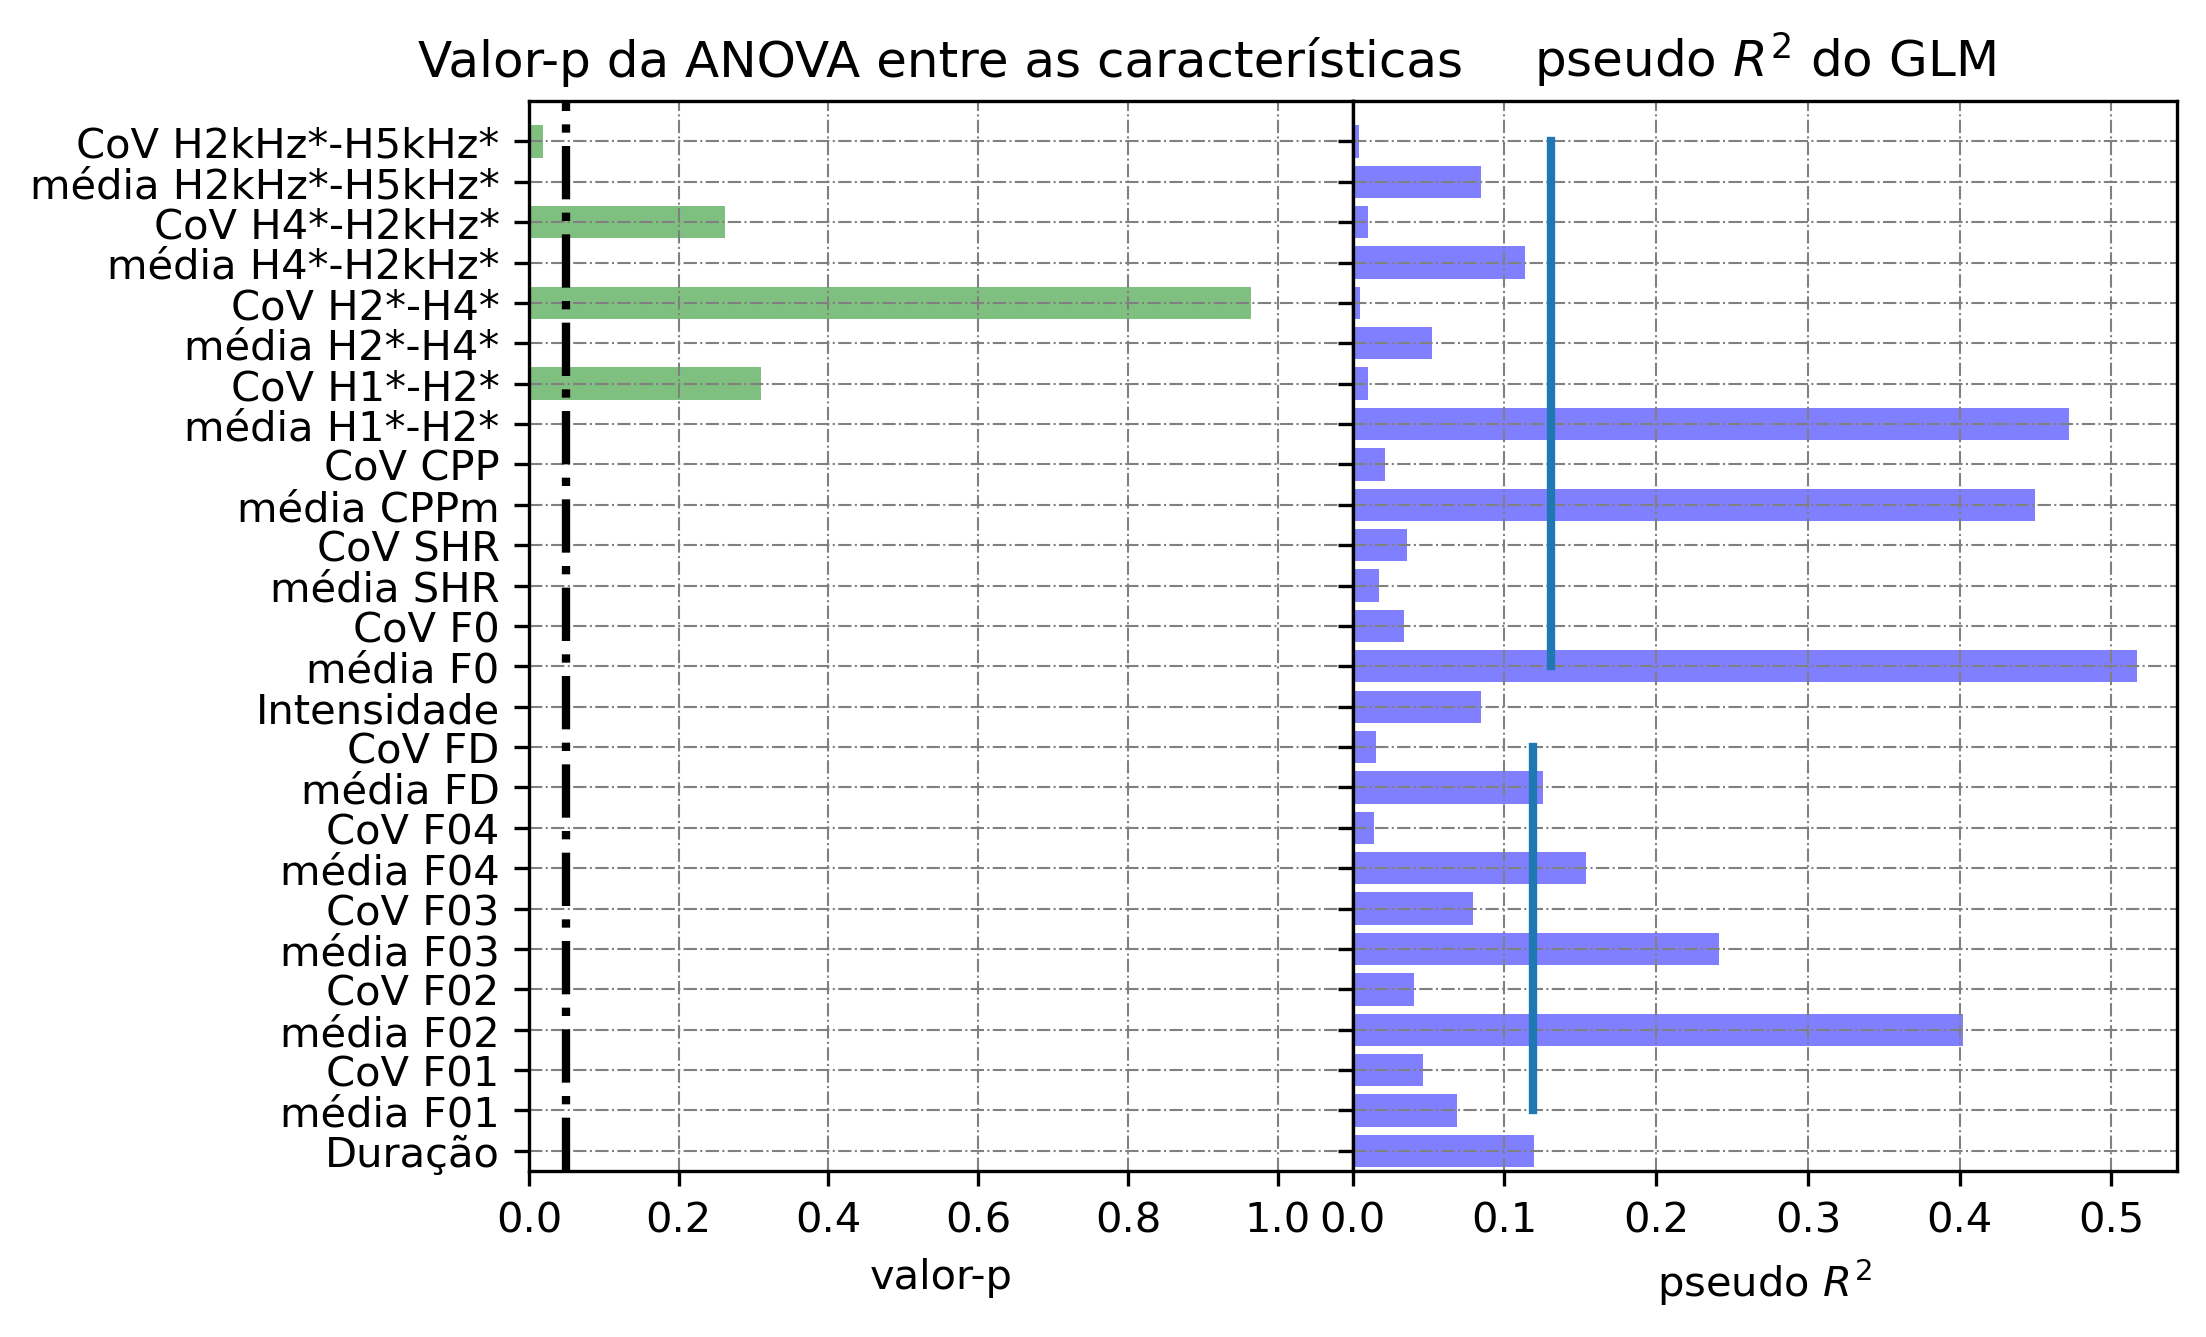
\includegraphics[height=7cm]{pValue_ANOVA_features.png}
				%		\caption{Autovalores normalizados da matriz de correlação.}
			\end{figure}
		\end{column}
	\end{columns}
\end{frame}

\begin{frame}[fragile=singleslide]
	\frametitle{Dispersão no espaço MDS}
	
	\begin{columns}
		\begin{column}{0.4\textwidth}
			Pseudo $R^2$ vocais vs. articulatórias\\
			\vspace{0.5cm}
			\textbf{Kolmogorov-Smirnov} falha em rejeitar que as distribuições são diferentes (valor-p de 0,31). \\
			\vspace{0.5cm}
			\textbf{Levene} falha em indicar a diferença de variância (valor-p de 0,59). \\
			\vspace{0.5cm}
			O \textbf{teste t} de diferença entre as médias falha (valor-p de 0,87).\\
		\end{column}
		\begin{column}{0.6\textwidth}  %%<--- here	
			\vspace{-1cm}
			\begin{figure}
				\centering
				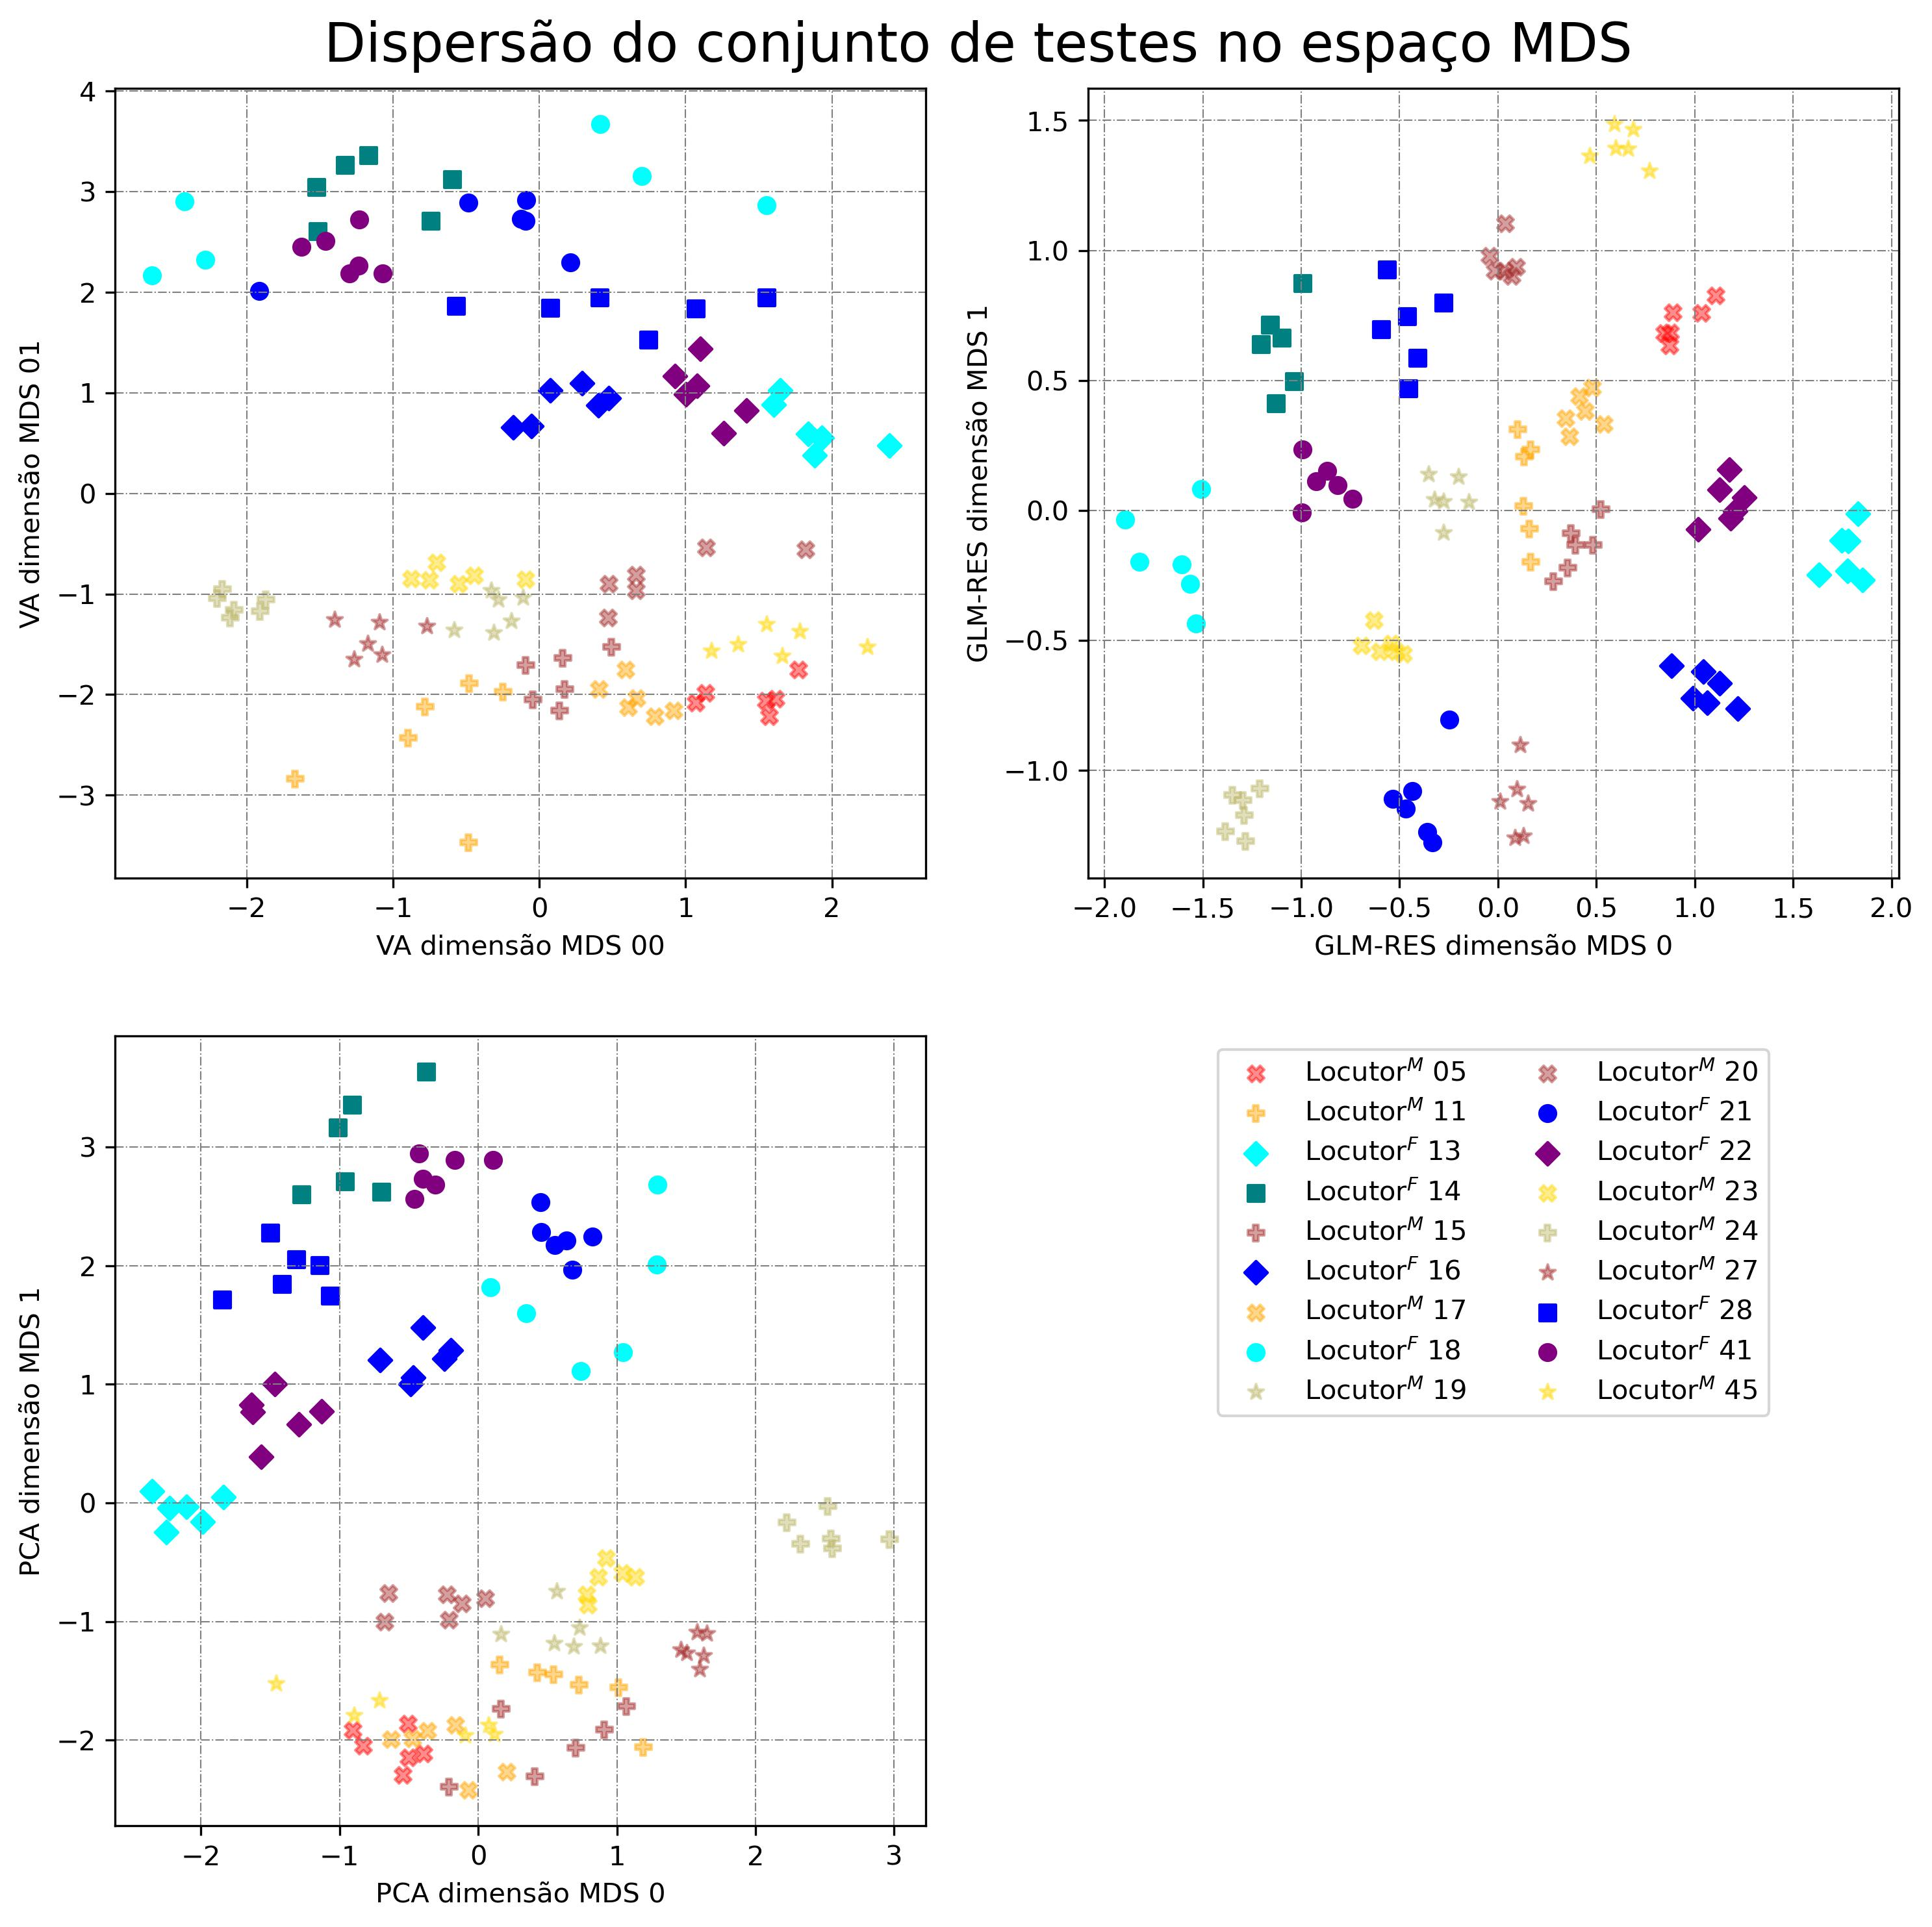
\includegraphics[height=7cm]{MDS_01.jpg}
				%		\caption{Autovalores normalizados da matriz de correlação.}
			\end{figure}
		\end{column}
		
	\end{columns}
\end{frame}

\begin{frame}[fragile=singleslide]
	\frametitle{Razão de dispersão}
	
	\begin{columns}
		\begin{column}{0.45\textwidth}			
			\textbf{Intralocutor}: $D_w$ distâncias de cada conjunto de vetores ao centroide.\\
			\vspace{0.5cm}
			
			\textbf{Interlocutor}: $D_b$ distância do centro da amostra a cada centroide de locutor normalizada pela distância do centroide mais distante$^*$.\\
			
%			\vspace{0.5cm}
			\[RD = \frac{D_w}{D_b} \]
		\end{column}
		\begin{column}{0.54\textwidth}  %%<--- here	
				\vspace{-1.0cm}
				\begin{figure}
				\centering
				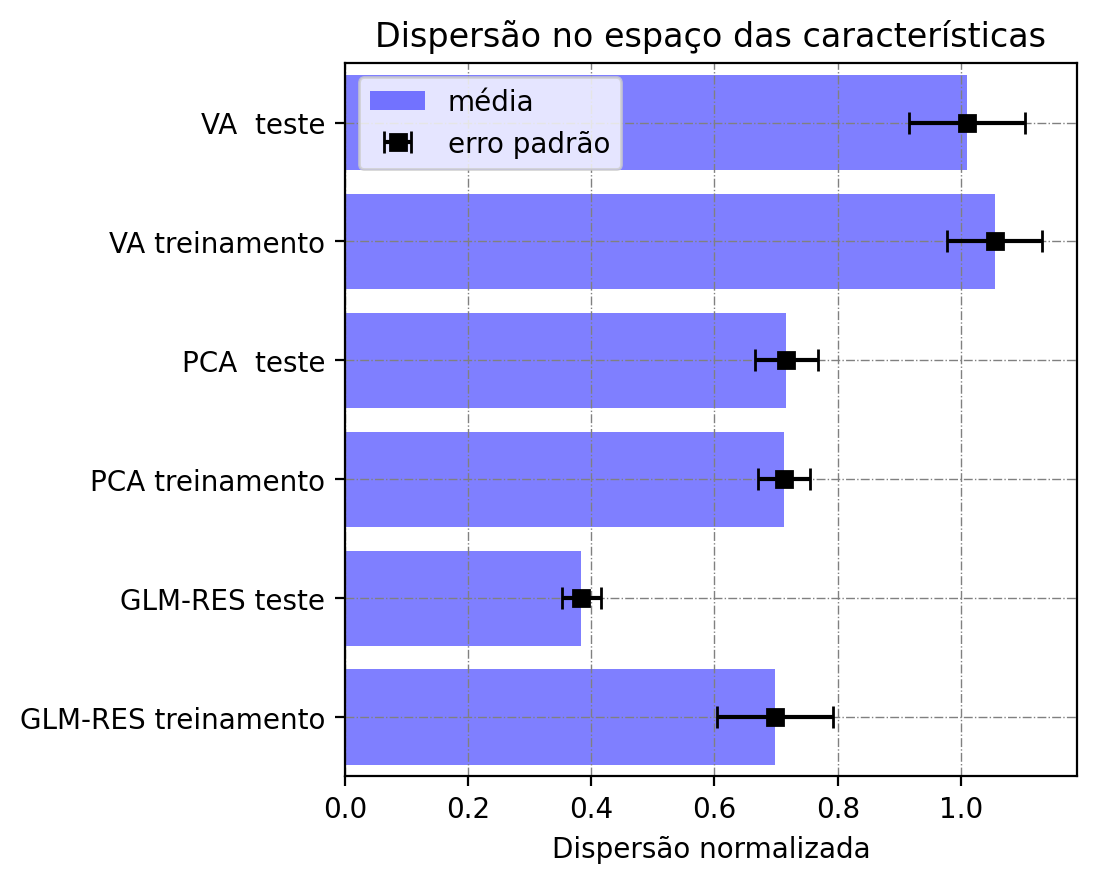
\includegraphics[height=5.9cm]{Dispersao.png}
%				\caption{Ocorrência das unidades amostrais por locutor.}
			\end{figure}			
		\end{column}
		
	\end{columns}
	\vfill
	* a normalização foi para fazer o ajuste da dimesionalidade.
	
\end{frame}



% ++++++++++++++++++++++++++++++++++++++++++++++++++++++++++++++++++++++++++++++
\subsection{Aplicação a comparação de locutores}
\begin{frame}[fragile=singleslide]
	\frametitle{Fluxograma das etapas de modelagem e comparação}
	\vspace{-0.35cm}
	\begin{figure}
		\centering
		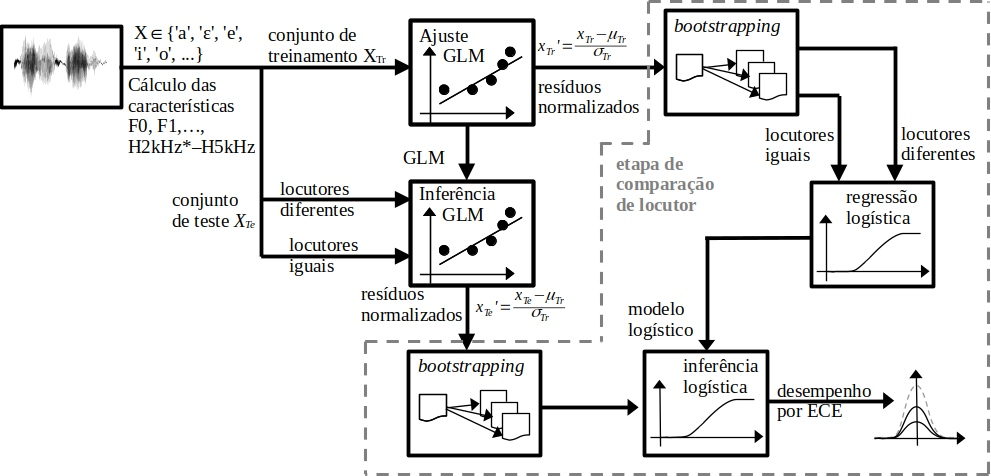
\includegraphics[height=7cm]{Fluxograma_v2.jpg}
		%		\caption{Autovalores normalizados da matriz de correlação.}
	\end{figure}
\end{frame}

\begin{frame}[fragile=singleslide]
	\frametitle{Etapas da comparação de locutor}
	A metodologia empregada para a comparação dos locutores é baseada nas etapas sequenciais: 
	\begin{enumerate}
		\item normalização do espaço pela média e desvio padrão dos dados;
		\item geração de duas subamostras, de treinamento e de testes obtidas por \textit{bootstrap};
		\item utilização da amostra de treinamento para o cálculo da distância euclidiana entre as subamostras indicando as comparações realizadas entre mesmo locutor e  locutores diferentes;
		\item ajuste de um modelo de regressão logística com base nas duas classes de comparações,  mesmo locutor e  locutores diferentes, utilizando o conjunto de treinamento; e 
		\item validação do modelo, com o conjunto de teste, e cálculo das métricas de desempenho.
	\end{enumerate}

\end{frame}

\begin{frame}[fragile=singleslide]
	\frametitle{Regressão logística}
	\begin{columns}
		\begin{column}{0.25\textwidth}
			\[LR = \frac{P(ML)}{P(LD)} \]
			\[LLR = \log_2 \left(\frac{P(ML)}{P(LD)} \right)\]
		\end{column}
		\begin{column}{0.75\textwidth}  %%<--- here	
			\vspace{-1.0cm}
			\begin{figure}
				\centering
				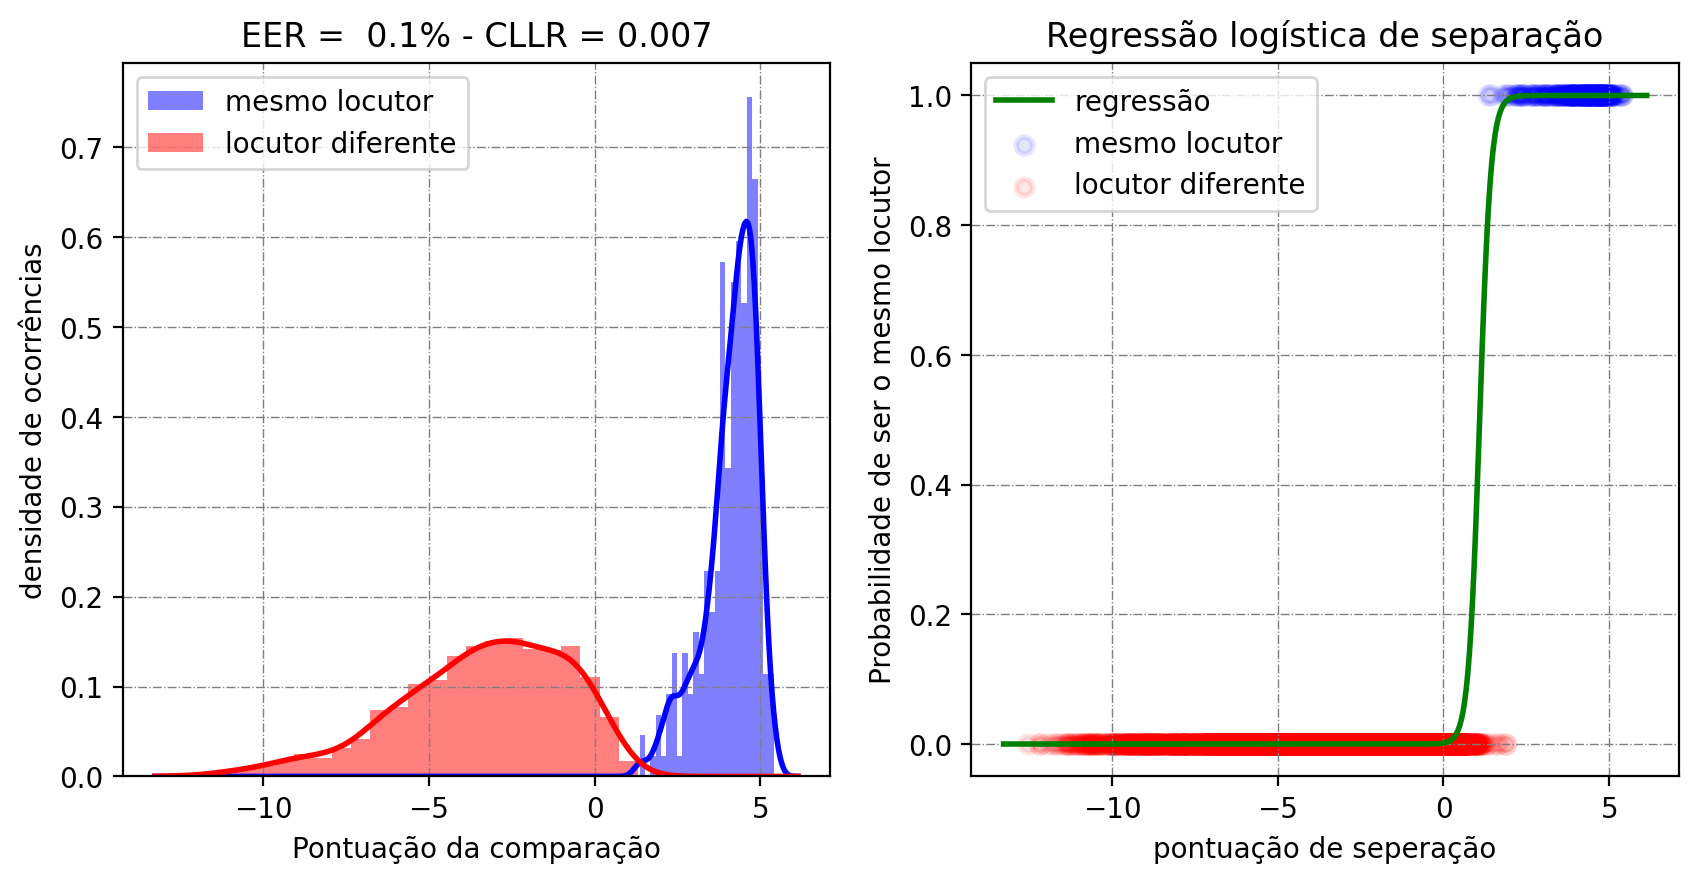
\includegraphics[height=6cm]{SMF_Logistic.png}
			\end{figure}
		\end{column}
	\end{columns}

\end{frame}

\begin{frame}[fragile=singleslide]
	\frametitle{Desempenho de ECE}
	\begin{columns}
		\begin{column}{0.45\textwidth}
			\textbf{Pontilhada cinza}: Classificador aleatório (LR = 1).\\
			\vspace{0.5cm}
			Quanto mais ``baixa'' menor o custo do erro na classificação.
			\begin{equation} \label{Hip_Hipotese_Anuncio}
				\begin{cases}
					H_0: & \text{Amostras locutores diferentes,}\\ \nonumber
					H_1: & \text{amostras do mesmo locutor.} 
				\end{cases}
			\end{equation}
		\end{column}
		\begin{column}{0.55\textwidth}  %%<--- here	
			\vspace{-1.0cm}
			\begin{figure}
				\centering
				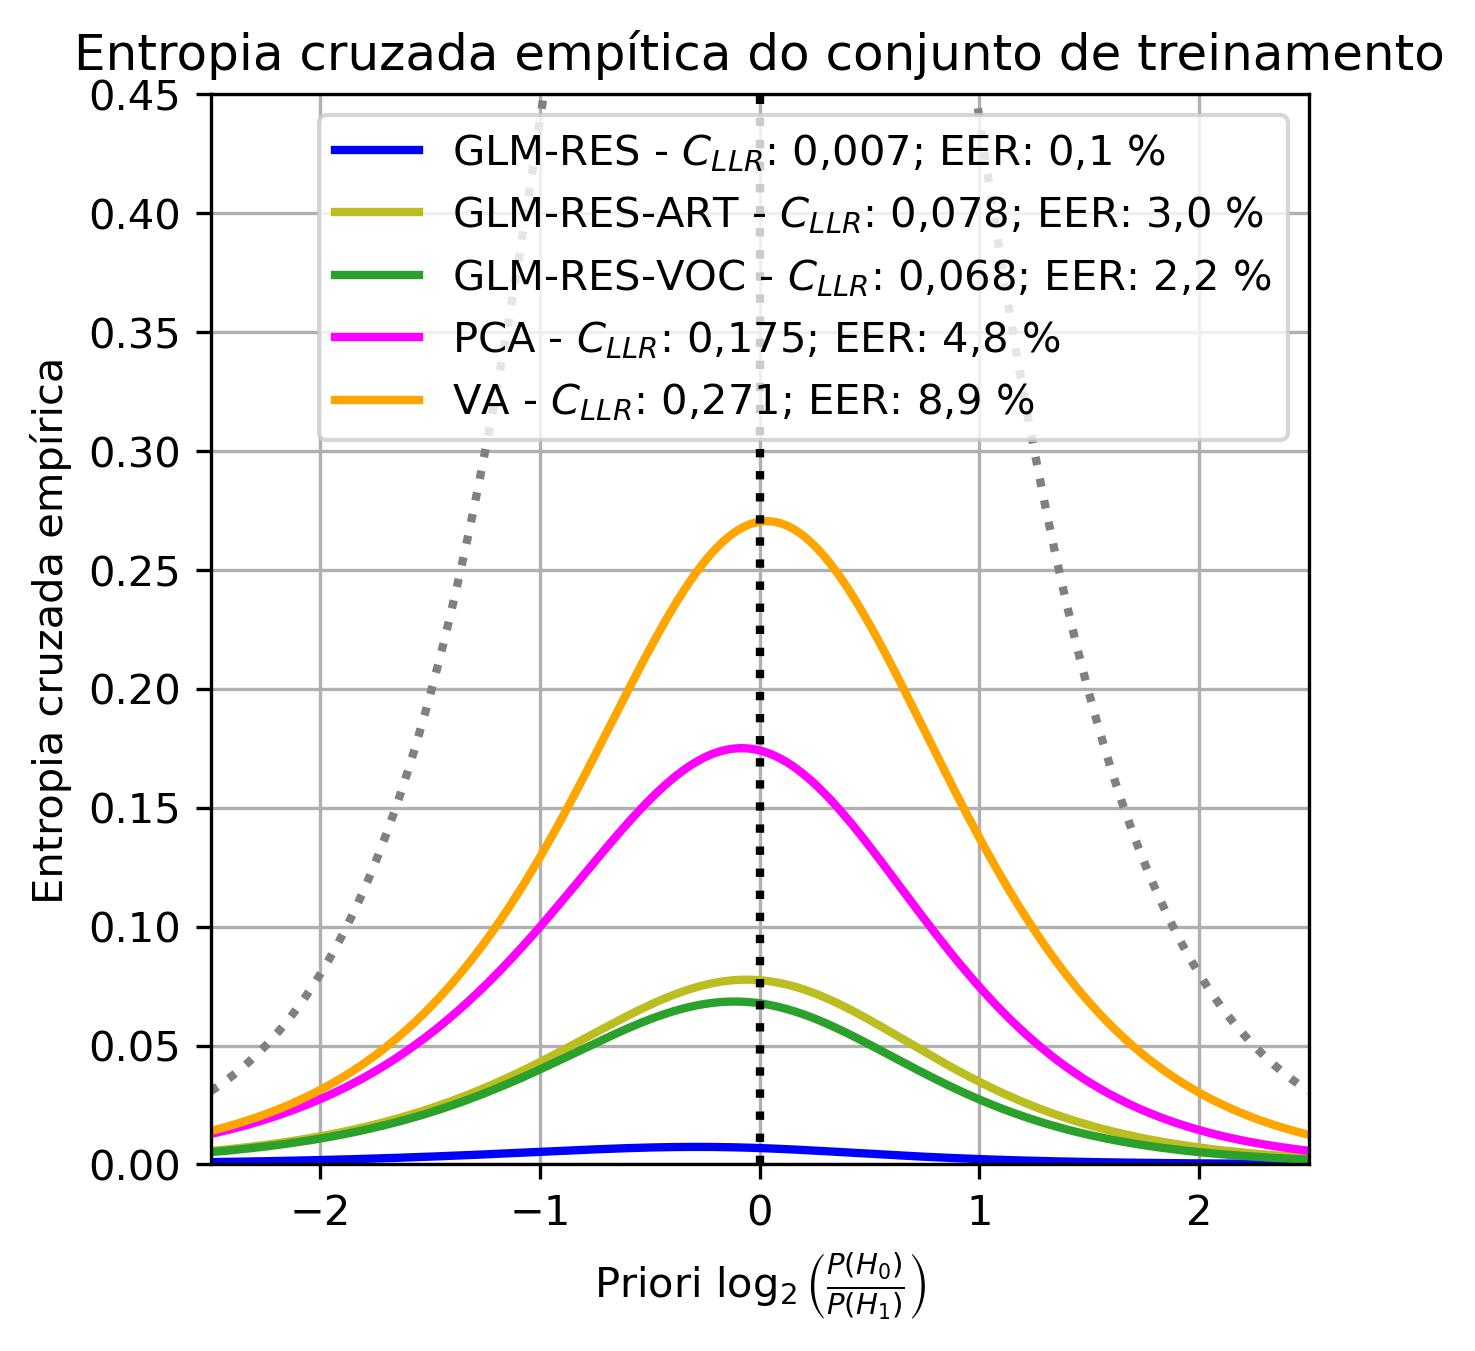
\includegraphics[height=6cm]{ECE_01.jpg}
			\end{figure}
		\end{column}
	\end{columns}
	\vfill
	\[ 
	C_{LLR} = \frac{1}{2} \left( \frac{1}{N_{ML}} \sum \log_{2} \left(1+ \frac{1}{LR_{MO}} \right) + \frac{1}{N_{LD}} \sum \log_{2} \left(1 + LR_{LD} \right) \right).
	\]
\end{frame}


\begin{frame}[fragile=singleslide]
	\frametitle{Resultados da comparação de locutor}
	Taxa de mesmo erro (EER - \textit{equal erro rate})\\
	$C_{LLR}$: Custo do logaritmo da razão de verossimilhança\\
	Entropia cruzada empírica (ECE - \textit{empirical cross entropy})\\
	TFP: Taxa de falso positivo (erro tipo I).\\
	TFN: Taxa de falso negativo (erro tipo II).
	
	\begin{table}[]
		\small
		\begin{tabular}{@{}l|cc|ccc@{}}
			\toprule
			\multirow{2}{*}{Espaço da medida acústica} & \multicolumn{2}{c|}{Treinamento} & \multicolumn{3}{c}{Teste (intervalo de confiança)}                            \\ \cmidrule(l){2-6}
			& EER (\%)       & $C_{LLR}$ (bits)       & Acurácia (\%)             & TFP (\%)                & TFN (\%)                \\ \midrule
			VA                                         & 8,9            & 0,271           & 89,8 (88,9; 90,6)         & 10,2 (9,3; 11,1)        & 10,0 (6,8; 13,2)        \\
			PCA                                        & 4,8            & 0,175           & 93,2 (92,7;93,8)          & 6,8 (6,2; 7,4)          & \textbf{5,8 (3,4; 8,3)} \\
			GLM-RES                                    & \textbf{0,1}   & \textbf{0,007}  & \textbf{99,1 (98,9;99,3)} & \textbf{0,6 (0,4; 0,8)} & 11,7 (9,6; 13,7)        \\
			GLM-RES-ART                                & 3              & 0,078           & 96,5 (96,1; 96,9)         & 3,0 (2,6; 3,4)          & 21,1 (18,5; 23,7)       \\
			GLM-RES-VOC                                & 2,2            & 0,068           & 96,9 (96,5; 97,2)         & 2,8 (2,5; 3,2)          & 12,2 (10,2; 14,2)       \\ \bottomrule
		\end{tabular}
	\end{table}
\end{frame}



\begin{frame}[fragile=singleslide]
	\frametitle{Análise de variância etapa de testes}
	\begin{figure}
		\centering
		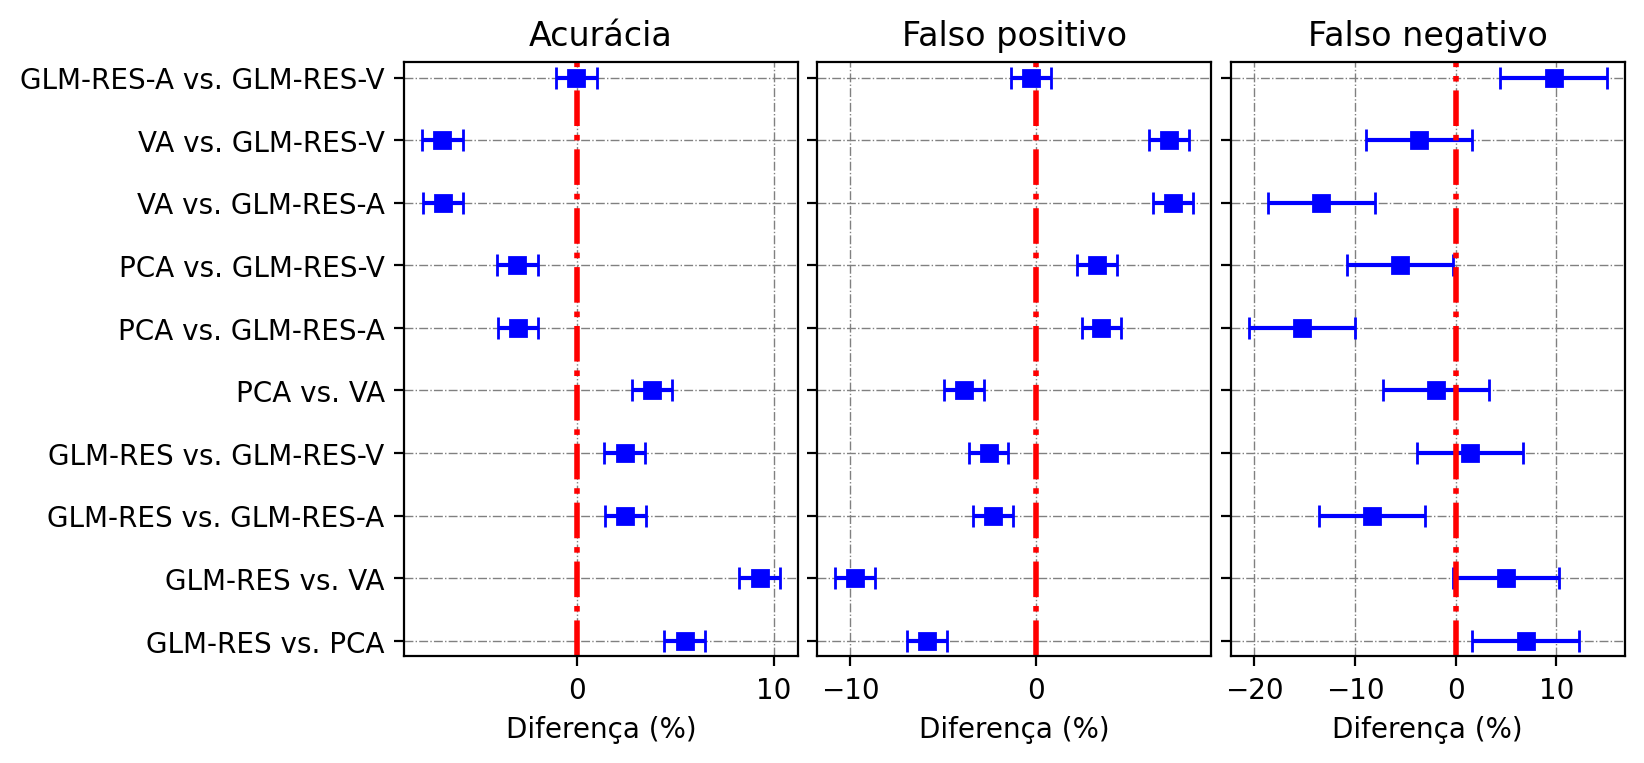
\includegraphics[height=7cm]{ANOVA_Acuracis_00.png}
		%		\caption{Autovalores normalizados da matriz de correlação.}
	\end{figure}
\end{frame}



% ==============================================================================
\section{Discussão}
\begin{frame}[fragile=singleslide]
	\frametitle{Principais achados}
	\textbf{Resultados}:
	\begin{itemize}
		\item O modelo GLM apresentou um pseudo R2 de 0,124.
		\item Redução da razão de dispersão: 63\% variáveis mensuráveis e de 46\% PCA. 
		\item Comparação de locutores com desempenho próximo ao estado da arte \cite{Sztaho2023,Ishihara2021}.
		\item Pior falso positivo em 11,7\% (101\% acima do melhor resultado), aumenta o \textit{in dubio pro reu}.
	\end{itemize}
	
	\textbf{Ainda pode-se avaliar}:
	\begin{itemize}
		\item Influência de cada variável de contexto;
		\item Influência das variáveis fictícias;
	\end{itemize}
\end{frame}
% ==============================================================================
\section{Considerações finais}
\begin{frame}[fragile=singleslide]
	\frametitle{Considerações finais}
	
	\textbf{Principais pontos:}
	\begin{itemize}
		\item No experimento específico foi eficiente em remover parte da variabilidade (++ hipótese);
		\item Foi eficiente na comparação dos locutores;
		\item Medidas vocais e articulatórias não apresentaram diferença significativa;
		\item Limitada na amostra de locutores e dialetos;
	\end{itemize}
	
	\textbf{Continuidade}:
	\begin{itemize}
		\item etiquetamento automatizado;
		\item expansão de dialetos;
		\item expandir contexto com cadência, prosódia, avaliação de emoção, etc...;
		\item expandir lista de medidas acústicas (e.g. \textit{cepstrun}).
	\end{itemize}
	
\end{frame}
% ==============================================================================

%% ------------------------------------------------------------------------
\section{Encerramento}
\frame{
	\frametitle{Agradecimentos}
	\vspace{-0.25cm}

	\begin{tikzpicture}[remember picture,overlay]
		\node[xshift=5.34cm,yshift=-3.25cm,opacity=1.0] at (current page.west) {
\includegraphics[height=1.25cm]{ADA_logo-borda.png}};
		\node[xshift=-3.125cm,yshift=-3.25cm,opacity=1.0] at (current page.east) {
\includegraphics[height=1.25cm]{logo_Acadepol_02.png}};
	\end{tikzpicture}

	\begin{center}
		\textbf{Fim!}
	\end{center}
	\vspace{-0.25cm}
	\begin{small}
		Contatos:
		\begin{itemize}
			\item e-mail: adelinocpp@gmail.com ou adelino.pinheiro@policiacivil.mg.gov.br;
			\item  Whatsapp (31) 98801-3605;
			\item Instituto de Criminologia - Academia de Polícia Civil de Minas Gerais. Rua Oscar Negrão de Lima n° 200, Nova Gameleira, Belo Horizonte-MG. Tel.: (31) 3314-5620.
		\end{itemize}
	\end{small}
}
%% ------------------------------------------------------------------------------
\begin{frame}[fragile=singleslide]
\frametitle{Sobre este material}
	Esta obra está licenciada sob a licença \href{http://creativecommons.org/licenses/by-nc-sa/4.0/}{\textit{Creative Commons} CC BY-NC-SA 4.0}\\
%
	\flushleft
	Favor fazer referência a este trabalho como:\linebreak

	\begin{small}
	Cantoni M. M., Silva, A. P., \textit{Modelagem estatística da variabilidade de inter e intrafalantes em fala contínua}. Online: {\url{https://github.com/adelinocpp/silf_2024}}
	\linebreak
	\begin{addmargin}[0.5cm]{0em}
		\begin{verbatim}
		@Misc{Cantoni2024,
		title={Modelagem estatística da variabilidade de inter e intrafalantes em fala contínua},
		author={Maria Mendes Cantoni and Adelino Pinheiro Silva},
		howPublished={\url{https://github.com/adelinocpp/silf_2024}},
		year={2024},
		note={Version 1.0; Creative Commons BY-NC-SA 4.0.},
		}
		\end{verbatim}
	\end{addmargin}
	\end{small}
	\vfill
	\begin{tikzpicture} [remember picture,overlay]
		\node[anchor=south,yshift=0.25cm] at (current page.south){ 
\includegraphics[width=.1\textwidth]{00BAS_CCsomerights.png}};
	\end{tikzpicture}
\end{frame}
%% ==============================================================================
\begin{frame}[allowframebreaks]
	\frametitle{Referências}
	\bibliographystyle{amsalpha}
	\bibliography{SILF_2024_v0.bib}
\end{frame}
%% ==============================================================================
\begin{frame}[fragile=singleslide]
	\frametitle{Dúvidas}
		\begin{tikzpicture}[remember picture,overlay]
		\node[xshift=0cm,yshift=-0.5cm,opacity=1.0] at (current page.center) {
\includegraphics[width=10cm]{principais-duvidas-sobre-o-trabalho-freelancer.jpg}};
	\end{tikzpicture}
	\vfill
	\lfr{Imagem: \url{https://www.hevcon.com.br/duvidas-frequentes-relacionado-ao-novo-bem-e-as-alteracoes-das-mps/}.}

\end{frame}
% ==============================================================================
\end{document}
